% Submission layout following the Taylor & Francis manuscript layout guide
% (Scandinavian Actuarial Journal): Times 12 pt, double spacing, line numbers,
% margins >= 2.5 cm, author-date references, statements before the references.
\documentclass[12pt]{article}
\usepackage[a4paper,margin=2.5cm]{geometry}
\usepackage[T1]{fontenc}
\usepackage{mathptmx}
\usepackage{setspace}
\usepackage[mathlines]{lineno}
\usepackage{microtype}
\usepackage{titlesec}
\usepackage{authblk}
\usepackage{amsmath,amssymb,amsthm}
\usepackage{natbib}
\usepackage{graphicx}
\usepackage{booktabs}
\usepackage[section]{placeins}
\usepackage{xcolor}
\usepackage[hidelinks]{hyperref}
\bibpunct{(}{)}{;}{a}{,}{,}

\newtheorem{theorem}{Theorem}[section]
\newtheorem{proposition}[theorem]{Proposition}
\newtheorem{lemma}[theorem]{Lemma}
\newtheorem{corollary}[theorem]{Corollary}
\theoremstyle{definition}
\newtheorem{definition}[theorem]{Definition}
\theoremstyle{remark}
\newtheorem{remark}[theorem]{Remark}

\newcommand{\todo}[1]{{\color{red}[#1]}}

% T&F heading levels: bold; bold italic; italic
\titleformat{\section}{\normalfont\large\bfseries}{\thesection.}{0.5em}{}
\titleformat{\subsection}{\normalfont\normalsize\bfseries\itshape}{\thesubsection.}{0.5em}{}
\titleformat{\subsubsection}{\normalfont\normalsize\itshape}{\thesubsubsection.}{0.5em}{}
\renewcommand\Authfont{\normalsize}
\renewcommand\Affilfont{\small\itshape}
\setlength{\emergencystretch}{1.5em}
\newcommand{\bF}{\overline{F}}
\newcommand{\E}{\mathrm{E}}
\newcommand{\PH}{\mathrm{PH}}
\newcommand{\EE}{\mathrm{EE}}
\newcommand{\VaR}{\mathrm{VaR}}
\DeclareMathOperator{\diag}{diag}

\title{Second-order behaviour of log phase-type tails and\\ threshold-robust tail index estimation}
\author[a]{Joseph H. T. Kim}
\author[b,c]{Himchan Jeong \thanks{Corresponding author. Email: himchanj@sfu.ca}}
\affil[a]{Department of Applied Statistics, Yonsei University, Seoul, Korea}
\affil[b]{Department of Statistics and Actuarial Science, Simon Fraser University, Burnaby, BC, Canada}
\affil[c]{Department of Next Generation Smart Energy System Convergence, Gachon University, Korea}
\date{}

\begin{document}
\maketitle
\doublespacing
\linenumbers

\begin{abstract}
\noindent Tail index estimates from the Hill estimator or from a generalised Pareto (GPD) fit to exceedances are notoriously sensitive to the threshold, because both ignore the second-order behaviour of the tail. Building on the eigenvalue plot of \citet{KimKim2015}, which fits a two-phase phase-type (PH$_2$) distribution to log-excesses, we show that a log-excess is PH$_2$ if and only if the loss tail is a signed two-Pareto mixture or a Pareto--log-gamma mixture, and that these tails are second-order regularly varying with $\rho<0$ and $\rho=0$, respectively. For the Pareto--log-gamma (Exp+Erlang) sub-model we derive the Fisher information in closed form; it is singular at the Pareto boundary, where the variance of the tail index estimator grows like $\xi^2/(4p^2)$ in the Erlang weight $p$. A simulation study with seven tail models shows that the Exp+Erlang sub-model gives the most threshold-robust tail index and high-quantile estimates in most settings, with profile-likelihood intervals close to nominal coverage where the fit is unbiased, while the Hill estimator remains preferable for nearly Pareto tails. The two-exponential sub-family is weakly identified, and $\rho$ cannot be recovered. We give closed-form expected shortfall and excess-of-loss layer premiums for the Exp+Erlang tail, with profile-likelihood intervals. For the Danish fire losses, the Exp+Erlang fit gives the most threshold-stable expected shortfall and layer premiums, reducing the model risk that the threshold choice introduces into capital and reinsurance calculations.
\end{abstract}

\noindent\textbf{Keywords:} Heavy tails; Hill estimator; phase-type distribution; second-order regular variation; threshold selection; Value-at-Risk

\noindent\textbf{MSC 2020:} 62G32; 60E05; 62F12; 62P05

\section{Introduction}\label{sec:intro}

Estimating the tail index of a heavy-tailed loss distribution is a routine but delicate task in insurance and finance. Its value determines which moments of the loss exist, and it drives the extrapolation behind high quantiles such as Value-at-Risk (VaR) and tail expectations. The two standard tools are the Hill estimator \citep{Hill1975} and maximum likelihood fitting of the generalised Pareto distribution (GPD) to the exceedances over a high threshold, the peaks-over-threshold (POT) method \citep{BalkemaDeHaan1974,Pickands1975,Smith1987,McNeil1997}. Both rely on the first-order approximation of the tail by a Pareto or GPD tail above the threshold, and both suffer from the same well-known difficulty: the estimate depends heavily on the threshold. A low threshold uses more data but incurs a bias from the part of the distribution where the first-order approximation is poor; a high threshold reduces this bias at the cost of a large variance \citep{Embrechts1997,Beirlant2004,ScarrottMacDonald2012}. The size of the bias is governed by the second-order behaviour of the tail, summarised by the second-order parameter $\rho\le 0$; when $\rho$ is close to zero the bias decays very slowly and no threshold gives a satisfactory trade-off \citep{Drees2000,DeHaanFerreira2006}.

A large literature reduces this sensitivity by modelling the second-order term explicitly, for example through the exponential regression model of \citet{Beirlant1999}, the Pareto-departure model of \citet{FeuervergerHall1999}, or bias-reduced estimators that plug in an external estimate of $\rho$ \citep{FragaAlves2003,GomesGuillou2015}. These methods are semi-parametric and target an asymptotic expansion of the tail.

For actuarial work the threshold problem is not only a statistical nuisance. Solvency capital at the 99.5\% level, expected shortfall and the pricing of high excess-of-loss reinsurance layers all depend on the fitted tail beyond the largest observations, and a threshold that is defensible on statistical grounds can still move these quantities substantially. The choice of threshold is therefore a source of model risk in capital and reinsurance calculations, and an estimator that is less sensitive to it, and that comes with honest uncertainty statements for the risk measures themselves, is of direct practical value.

A different, fully parametric route was proposed by \citet{KimKim2015}, motivated by the log phase-type (LogPH) class of \citet{Ahn2012}. If a loss $Y$ has a regularly varying tail, the log-excess $\log(Y/u)$ over a threshold $u$ has an exponentially decaying distribution, and the Hill estimator is the exponential maximum likelihood estimator (MLE) for these log-excesses. \citet{KimKim2015} replaced the exponential by a phase-type distribution with two phases, PH$_2$, fitted by the EM algorithm of \citet{Asmussen1996}, and plotted the resulting tail index (the eigenvalue of the PH generator closest to zero) against the threshold. Their eigenvalue plot was markedly more stable than the Hill plot across the examples they considered. Two questions were left open: what PH$_2$ fitting implies for the second-order behaviour of the tail, and whether the gain in stability holds up in a systematic comparison that includes the GPD.

This paper answers both questions, and our conclusions are partly positive and partly negative. Our contributions are as follows.
\begin{enumerate}
\item We give an explicit characterisation of PH$_2$ with exact parameter ranges (Proposition~\ref{prop:ph2}). A PH$_2$ law is either a signed mixture of two exponentials, which we call the two-exponential (2E) sub-family, or a mixture of an exponential and an Erlang(2) law with the same rate, the Exp+Erlang (EE) sub-family; each has a Coxian representation, and EE is a boundary limit of 2E. For losses this means that the tail beyond the threshold is either a signed two-Pareto mixture or a Pareto--log-gamma mixture.
\item We show that both log-tails are second-order regularly varying, with $\rho=-\tau$ for 2E and $\rho=0$ for EE, and we give the auxiliary functions in closed form (Theorem~\ref{thm:2rv}). Hence log-PH$_2$ tails cover every $\rho\le 0$. We derive the exact bias of the Hill functional under each case and contrast it with the threshold invariance of the PH$_2$ rate parameters (Proposition~\ref{prop:hill}).
\item For the EE sub-model, a two-parameter generalisation of the Hill model, we derive the Fisher information in closed form via the exponential integral (Proposition~\ref{prop:fisher}). We show that it is singular at the Pareto boundary $p=0$, with $\det I=4p^2/\mu^2+O(p^3)$, so that the variance of the tail index estimator grows like $\xi^2/(4p^2)$ (Proposition~\ref{prop:singular}). This explains both the cost of the extra flexibility near an exact Pareto tail and the difficulty of identifying $\rho$, and it motivates profile-likelihood intervals.
\item In a simulation study with seven tail models, two sample sizes and 500 replications, we compare Hill, GPD and several PH$_2$ variants over a wide range of thresholds (Section~\ref{sec:sim}). The EE sub-model gives the flattest error curves across thresholds and the smallest best-threshold error for most models, while the Hill estimator remains best for tails close to an exact Pareto. The 2E sub-family degrades accuracy when selected, and information criteria do not recover the second-order case.
\item For actuarial use we give closed-form stop-loss transforms, mean excess functions, expected shortfall and excess-of-loss layer premiums under the EE tail, and profile-likelihood intervals for these quantities (Section~\ref{sec:risk}). Applied to the Danish fire losses, the EE fit gives the most threshold-stable expected shortfall and layer premiums of the three methods, and its intervals for expected shortfall are narrower than those of the GPD (Section~\ref{sec:data}). The fitted Erlang weight also gives a practical diagnostic for when the classical Pareto (Hill) tail is adequate.
\end{enumerate}

The paper is organised as follows. Section~\ref{sec:background} reviews regular variation, the Hill and POT approaches and phase-type distributions. Section~\ref{sec:ph2} characterises PH$_2$ and the corresponding log-tails, and Section~\ref{sec:2rv} studies their second-order behaviour. Section~\ref{sec:inference} develops likelihood inference for the EE sub-model, and Section~\ref{sec:risk} derives tail risk measures and reinsurance layer premiums with interval estimates. Section~\ref{sec:sim} reports the simulation study and Section~\ref{sec:data} an empirical illustration. Section~\ref{sec:discussion} gives practical recommendations and discusses limitations. Proofs are collected in Appendix~\ref{app:proofs}.

\section{Background}\label{sec:background}

\subsection{First- and second-order regular variation}

Let $Y>0$ be a loss with distribution function $F$ and tail $\bF=1-F$. The tail is regularly varying with index $-\alpha<0$, written $\bF\in RV_{-\alpha}$, if
\begin{equation}\label{eq:rv}
\lim_{t\to\infty}\frac{\bF(tx)}{\bF(t)}=x^{-\alpha},\qquad x>0.
\end{equation}
Equivalently, $\bF(y)=y^{-\alpha}L(y)$ with $L$ slowly varying. We call $\alpha$ the tail index and write $\xi=1/\alpha$ for the extreme value index; moments of order less than $\alpha$ are finite.

The rate of convergence in \eqref{eq:rv} is described by second-order regular variation \citep{Geluk1997,DeHaanFerreira2006}.

\begin{definition}\label{def:2rv}
$\bF$ is second-order regularly varying with first-order index $-\alpha$ and second-order parameter $\rho\le 0$, written $\bF\in 2RV_{-\alpha,\rho}$, if there is a function $A(t)\to0$ of ultimately constant sign such that
\begin{equation}\label{eq:2rv}
\lim_{t\to\infty}\frac{\bF(tx)/\bF(t)-x^{-\alpha}}{A(t)}=x^{-\alpha}\,\frac{x^{\rho}-1}{\rho},\qquad x>0,
\end{equation}
where the right-hand side is read as $x^{-\alpha}\log x$ when $\rho=0$. Then $|A|\in RV_{\rho}$.
\end{definition}

We use the tail-function scale for $\rho$ throughout. If $\bF\in 2RV_{-\alpha,\rho}$, then the tail quantile function $U(t)=F^{\leftarrow}(1-1/t)$ is second-order regularly varying with first-order index $\xi$ and second-order parameter $\rho/\alpha$ where $F^{\leftarrow}(q)=\inf\{y: F(y)\ge q\}$ denotes the generalised inverse (quantile function) of $F$; the latter is the scale on which $\rho$ is usually reported in the statistics literature \citep{DeHaanFerreira2006}. The parameter $\rho$ governs the bias of tail index estimators: for the Hill estimator based on the $k$ largest observations, the asymptotic bias is proportional to $A(n/k)$-type terms, which decay only logarithmically when $\rho=0$ \citep{Drees2000,Beirlant2004}.

\subsection{The Hill estimator and the POT method}

Let $Y_{1:n}\le\dots\le Y_{n:n}$ be the order statistics of a sample of size $n$, and let $u=Y_{n-k:n}$ be the threshold leaving $k$ exceedances. Writing $E_j=\log(Y_{n-j+1:n}/u)$, $j=1,\dots,k$, for the log-excesses, the Hill estimator is
\begin{equation}\label{eq:hill}
\hat\xi^{H}_k=\frac1k\sum_{j=1}^k E_j .
\end{equation}
If $\bF$ is exactly Pareto above $u$, the log-excesses are i.i.d.\ exponential with mean $\xi$, and \eqref{eq:hill} is the exponential MLE. For high quantiles we use the estimator of \citet{Weissman1978}, $\widehat{\VaR}_p=u\{n(1-p)/k\}^{-\hat\xi^H_k}$.

The POT method fits the GPD with shape $\xi$ and scale $\sigma$ to the excesses $Y-u$ by maximum likelihood \citep{Smith1987,McNeil1997}, and estimates $\VaR_p$ by $u+\hat\sigma\hat\xi^{-1}[\{n(1-p)/k\}^{-\hat\xi}-1]$. Its approximation error above $u$ is governed by the same second-order function $A$ \citep{DeHaanFerreira2006}.

\subsection{Phase-type and log phase-type distributions}

A random variable $X\ge0$ has a phase-type distribution $\PH(\beta,T)$ with $m$ phases if it is the absorption time of a continuous-time Markov chain with $m$ transient states, initial distribution $\beta$ (a row vector with $\beta\mathbf 1=1$) and sub-generator $T$ \citep{Neuts1981,BladtNielsen2017}. Its survival function and density are
\begin{equation}\label{eq:ph}
\Pr(X>x)=\beta e^{Tx}\mathbf 1,\qquad f(x)=\beta e^{Tx}t,\quad t=-T\mathbf 1,\qquad x\ge 0.
\end{equation}
All eigenvalues of $T$ have negative real parts. If $-\eta_T$ denotes the eigenvalue with the largest real part and $\beta$ charges the corresponding eigenspace, then $\Pr(X>x)$ decays like $x^{j}e^{-\eta_T x}$ for some integer $j\ge 0$.

Phase-type laws are closed under excess: for $d\ge 0$,
\begin{equation}\label{eq:excess}
X-d\mid X>d\ \sim\ \PH(\beta_d,T),\qquad \beta_d=\frac{\beta e^{Td}}{\beta e^{Td}\mathbf 1}.
\end{equation}
The sub-generator $T$, and hence $\eta_T$, does not depend on $d$; only the initial vector moves.

Following \citet{Ahn2012} and \citet{KimKim2015}, we say that $Y$ has a log phase-type tail above $u_0$ if $\log(Y/u_0)\mid Y>u_0\sim\PH(\beta,T)$. By \eqref{eq:excess}, $\log(Y/u)\mid Y>u\sim\PH(\beta_{\log(u/u_0)},T)$ for every $u\ge u_0$. In particular, $\bF\in RV_{-\eta_T}$ (possibly with a power-of-log factor), so $\eta_T$ is the tail index whatever the threshold. This threshold stability, the PH analogue of the GPD threshold stability, is the basis of the eigenvalue plot of \citet{KimKim2015}: one fits $\PH(\beta,T)$ to the log-excesses over a range of thresholds and plots $1/\hat\eta_T$. Note that $m=1$ gives back the Hill estimator.

\section{The two-phase class and its log-tails}\label{sec:ph2}

With $m=2$ phases the class is small enough to be described completely, and this description is the key to everything that follows. \citet{DicksonHipp2000} observed that a PH$_2$ law is either a combination of two exponentials or a combination of an exponential and an Erlang(2) law. We make this precise, including the exact parameter ranges.

\begin{lemma}\label{lem:eigen}
The eigenvalues of a $2\times 2$ sub-generator are real and negative.
\end{lemma}

\begin{proposition}\label{prop:ph2}
A random variable $X\ge 0$ with no atom at zero is $\PH_2$ distributed if and only if its survival function $S(x)=\Pr(X>x)$ has one of the following two forms:
\begin{enumerate}
\item[\textup{(2E)}] for some $\theta>0$, $\tau>0$ and $-\theta/\tau\le w\le 1$,
\begin{equation}\label{eq:2E}
S(x)=(1-w)e^{-\theta x}+w\,e^{-(\theta+\tau)x},\qquad f(x)=(1-w)\theta e^{-\theta x}+w(\theta+\tau)e^{-(\theta+\tau)x};
\end{equation}
\item[\textup{(EE)}] for some $\mu>0$ and $0\le p\le 1$,
\begin{equation}\label{eq:EE}
S(x)=e^{-\mu x}(1+p\mu x),\qquad f(x)=(1-p)\mu e^{-\mu x}+p\,\mu^2xe^{-\mu x}.
\end{equation}
\end{enumerate}
Case \textup{(2E)} arises when $T$ has two distinct eigenvalues $-\theta$ and $-(\theta+\tau)$; case \textup{(EE)} arises when $T$ has a double eigenvalue $-\mu$. Conversely, every law in \eqref{eq:2E} is $\PH_2$ with the Coxian representation
\begin{equation}\label{eq:cox2E}
\beta=(1,0),\qquad T=\begin{pmatrix}-(\theta+\tau) & q(\theta+\tau)\\ 0 & -\theta\end{pmatrix},\qquad q=\frac{(1-w)\tau}{\theta+\tau}\in[0,1],
\end{equation}
and every law in \eqref{eq:EE} is $\PH_2$ with $\beta=(1,0)$ and $T=\begin{pmatrix}-\mu & p\mu\\ 0&-\mu\end{pmatrix}$.
\end{proposition}

The weight $w$ in \eqref{eq:2E} may be negative: for $-\theta/\tau\le w<0$ the density is hump-shaped (hypo-exponential), while for $0<w<1$ it is a genuine hyperexponential mixture. The tail rate is $\theta$ whenever $w<1$. In the (EE) case the tail rate is $\mu$, and $p=0$ gives the exponential law of the Hill model.

\begin{remark}[EE as a boundary of 2E]\label{rem:limit}
Put $w=-p\theta/\tau$ in \eqref{eq:2E}. Then $S(x)=e^{-\theta x}\{1+p\theta(1-e^{-\tau x})/\tau\}\to e^{-\theta x}(1+p\theta x)$ as $\tau\downarrow 0$, which is \eqref{eq:EE} with $\mu=\theta$. The constraint $w\ge-\theta/\tau$ becomes $p\le 1$. Thus the EE sub-family lies on the boundary $\tau=0$ of the 2E sub-family. Testing EE against 2E is therefore a boundary problem with a nuisance parameter, and standard likelihood-ratio or information-criterion calibrations do not apply \citep{SelfLiang1987}. We return to this in Section~\ref{sec:selection}.
\end{remark}

By the threshold stability \eqref{eq:excess}, each sub-family is closed under excess with the same rates, only the weight changing:
\begin{equation}\label{eq:weights}
w_d=\frac{w e^{-\tau d}}{1-w+we^{-\tau d}}\quad\text{(2E)},\qquad p_d=\frac{p}{1+p\mu d}\quad\text{(EE)}.
\end{equation}

Translating to losses gives the two possible log-PH$_2$ tails.

\begin{corollary}\label{cor:tails}
Suppose $\log(Y/u_0)\mid Y>u_0\sim\PH_2$. Then for $y\ge u_0$, the conditional tail $\bF_{u_0}(y)=\Pr(Y>y\mid Y>u_0)$ is either
\begin{align}
\bF_{u_0}(y)&=(1-w)\Big(\frac{y}{u_0}\Big)^{-\theta}+w\Big(\frac{y}{u_0}\Big)^{-(\theta+\tau)} &&\text{(signed two-Pareto mixture)},\label{eq:tail2E}\\
\bF_{u_0}(y)&=\Big(\frac{y}{u_0}\Big)^{-\mu}\Big\{1+p\mu\log\frac{y}{u_0}\Big\} &&\text{(Pareto--log-gamma mixture)}.\label{eq:tailEE}
\end{align}
The law in \eqref{eq:tailEE} mixes, with weights $1-p$ and $p$, a Pareto law with index $\mu$ and a log-gamma law with shape $2$ and rate $\mu$, both supported on $[u_0,\infty)$.
\end{corollary}

\section{Second-order behaviour}\label{sec:2rv}

The two tails in Corollary~\ref{cor:tails} share the first-order index but differ at second order. The second-order condition \eqref{eq:2rv} holds for them exactly, not only asymptotically.

\begin{theorem}\label{thm:2rv}
Let $\bF$ have a log-$\PH_2$ tail above $u_0$, and write $s=\log(t/u_0)$ for $t\ge u_0$.
\begin{enumerate}
\item[(a)] In case \textup{(EE)} with $0<p\le1$, $\bF\in 2RV_{-\mu,0}$ with
\begin{equation}\label{eq:AEE}
\begin{gathered}
A(t)=\frac{p\mu}{1+p\mu s}\sim\frac{1}{\log t},\\
\frac{\bF(tx)}{\bF(t)}-x^{-\mu}=A(t)\,x^{-\mu}\log x\qquad\text{for all } t\ge u_0,\ x\ge1 .
\end{gathered}
\end{equation}
\item[(b)] In case \textup{(2E)} with $w<1$ and $w\ne0$, $\bF\in 2RV_{-\theta,-\tau}$ with
\begin{equation}\label{eq:A2E}
\begin{gathered}
A(t)=\frac{-\tau w e^{-\tau s}}{1-w+we^{-\tau s}},\\
\frac{\bF(tx)}{\bF(t)}-x^{-\theta}=A(t)\,x^{-\theta}\,\frac{x^{-\tau}-1}{-\tau}\qquad\text{for all } t\ge u_0,\ x\ge1 .
\end{gathered}
\end{equation}
The sign of $A$ is that of $-w$, and $|A|\in RV_{-\tau}$.
\item[(c)] If $p=0$ in \textup{(EE)} or $w=0$ in \textup{(2E)}, the tail is exactly Pareto above $u_0$ and the left-hand side of \eqref{eq:2rv} vanishes identically.
\end{enumerate}
\end{theorem}

\begin{corollary}\label{cor:range}
The second-order parameters attained by log-$\PH_2$ tails are exactly $\rho\in(-\infty,0]$, together with the exact Pareto tail. The value $\rho=0$ is attained only in case \textup{(EE)}, and every $\rho<0$ only in case \textup{(2E)} with $\tau=-\rho$.
\end{corollary}

Case (2E) belongs to the class of \citet{Hall1982}, $\bF(y)=Cy^{-\alpha}\{1+Dy^{\rho}+o(y^{\rho})\}$, and is the convex (or signed) Pareto mixture considered by \citet{FeuervergerHall1999}. Case (EE) is the canonical $\rho=0$ tail: its slowly varying part is $1+p\mu\log(y/u_0)$, a log factor of the kind that makes the Hill estimator converge slowly.

The next result makes the contrast with the Hill estimator concrete. Let $L(u)=\E[\log(Y/u)\mid Y>u]$ be the population version of the Hill estimator at threshold $u$.

\begin{proposition}\label{prop:hill}
Under a log-$\PH_2$ tail above $u_0$, the log-excess over any $u\ge u_0$ stays in the same sub-family with the same rate parameters, and only the weight changes as in \eqref{eq:weights} with $d=\log(u/u_0)$. The Hill functional satisfies:
\begin{enumerate}
\item[(a)] in case \textup{(EE)}, $L(u)=\xi(1+p_d)$ with $\xi=1/\mu$, so the bias is $L(u)-\xi=\xi p_d\sim \xi^2/\log u$;
\item[(b)] in case \textup{(2E)}, $L(u)=\xi-\xi\,w_d\,\tau/(\theta+\tau)$ with $\xi=1/\theta$, so the bias is $O(u^{-\tau})=O(u^{\rho})$.
\end{enumerate}
In contrast, the MLE of $\mu$ (or of $\theta$) in the correctly specified $\PH_2$ sub-model is consistent for the tail index at every fixed threshold $u\ge u_0$.
\end{proposition}

Proposition~\ref{prop:hill} formalises the mechanism behind the eigenvalue plot. Under an EE tail, the Hill bias decays only like $1/\log u$, so lowering the threshold to gain data is heavily penalised. The PH$_2$ fit absorbs the slowly varying factor into the weight $p_d$, which is re-estimated at each threshold, and the rate parameter is threshold-invariant. This argument is exact only inside the model. Outside it, for example under a log-gamma tail with non-integer shape or a Burr tail, the EE fit can at best absorb the second-order term locally, and its bias must be assessed empirically (Section~\ref{sec:sim}).

\section{Likelihood inference for the EE sub-model}\label{sec:inference}

\subsection{Estimation}

Given log-excesses $E_1,\dots,E_k$ over $u$, the EE log-likelihood is
\begin{equation}\label{eq:loglik}
\ell(\mu,p)=k\log\mu-\mu\sum_{j=1}^kE_j+\sum_{j=1}^k\log(1-p+p\mu E_j),\qquad \mu>0,\ 0\le p\le1 .
\end{equation}
At $p=0$ it reduces to the exponential log-likelihood, whose maximiser is the Hill estimator. We maximise \eqref{eq:loglik} directly, using a logistic transform for $p$, analytic gradients and several starting values. The 2E likelihood is handled in the same way, with $w=-\theta/\tau+(1+\theta/\tau)\,\mathrm{expit}(c)$ (Appendix~\ref{app:computing}). Direct maximisation of the explicit densities of Proposition~\ref{prop:ph2} targets the same estimator as the EM algorithm used by \citet{KimKim2015}, is considerably faster, and returns the fitted sub-family. The tail index estimate is $\hat\xi=1/\hat\mu$, and a high quantile is estimated by $u\exp\{S^{-1}_{\hat\mu,\hat p}(n(1-p_{\mathrm{VaR}})/k)\}$, with $S$ from \eqref{eq:EE}.

\subsection{Fisher information and its singularity at the Pareto boundary}

Let $E_1(a)=\int_a^\infty e^{-s}s^{-1}\,ds$ denote the exponential integral \citep{AbramowitzStegun1964}.

\begin{proposition}\label{prop:fisher}
For $0<p<1$, put $a=(1-p)/p$ and $J=e^{a}E_1(a)$. The per-observation Fisher information of the EE model \eqref{eq:EE} is
\begin{equation}\label{eq:fisher}
I(\mu,p)=\begin{pmatrix}
\dfrac{1+p(1-a+a^2J)}{\mu^2} & -\dfrac{1-aJ}{\mu p}\\[2ex]
-\dfrac{1-aJ}{\mu p} & \dfrac{J-p}{p^{3}}
\end{pmatrix}.
\end{equation}
For $0<p<1$ the MLE is asymptotically normal, $\sqrt k(\hat\xi-\xi)\Rightarrow N(0,\sigma^2_\xi(p))$, with $\sigma^2_\xi(p)=\xi^4\,[I(\mu,p)^{-1}]_{11}$. The ratio $\sigma^2_\xi(p)/\xi^2$ depends on $p$ only.
\end{proposition}

We verified \eqref{eq:fisher} against Monte Carlo estimates of the score covariance to three significant digits. Table~\ref{tab:infl} reports the variance of $\hat\xi$ relative to $\xi^2$, the asymptotic variance of the Hill estimator under an exact Pareto tail. The extra parameter is cheap when the Erlang component is substantial, but becomes very expensive as $p\downarrow 0$.

\begin{table}[t]
\centering
\small
\caption{Asymptotic variance of the Exp+Erlang MLE $\hat\xi$, relative to $\xi^2$ (the asymptotic variance of the Hill estimator under an exact Pareto tail), as a function of the Erlang weight $p$.}
\label{tab:infl}
\begin{tabular}{lrrrrrrr}
\toprule
$p$ & 0.05 & 0.10 & 0.20 & 0.30 & 0.50 & 0.70 & 0.90 \\
\midrule
$\sigma^2_\xi(p)/\xi^2$ & 118.23 & 33.50 & 10.07 & 5.12 & 2.21 & 1.25 & 0.78 \\
\bottomrule
\end{tabular}
\end{table}


\begin{proposition}\label{prop:singular}
As $p\downarrow0$, $I(\mu,p)\to I_0=\begin{pmatrix}\mu^{-2}&-\mu^{-1}\\-\mu^{-1}&1\end{pmatrix}$, which is singular. More precisely, $\det I(\mu,p)=4p^2/\mu^2+O(p^3)$ and
\begin{equation}\label{eq:blowup}
\frac{\sigma^2_\xi(p)}{\xi^2}=\frac{1}{4p^2}\{1+O(p)\}.
\end{equation}
At $p=0$ the two scores are collinear: $\partial_p\ell=-\mu\,\partial_\mu\ell=\mu E-1$.
\end{proposition}

At the Pareto boundary, the EE model therefore has a singular information matrix with the true parameter on the edge of the parameter space. Standard $\sqrt k$ asymptotics fail there \citep{SelfLiang1987,Rotnitzky2000}. To first order, a small Erlang component cannot be told apart from a small change in the tail rate. This is the precise sense in which the departure from an exact Pareto tail, and hence the second-order case, is hard to identify, and it is consistent with the selection behaviour in Section~\ref{sec:sim}.

\subsection{Confidence intervals}

Wald intervals based on \eqref{eq:fisher} inherit the singularity: when $\hat p$ is small they become extremely wide or numerically undefined. We therefore recommend the profile-likelihood interval
\begin{equation}\label{eq:profile}
\Big\{\xi=1/\mu:\ 2\big[\ell(\hat\mu,\hat p)-\max_{0\le p\le1}\ell(\mu,p)\big]\le\chi^2_{1,0.95}\Big\},
\end{equation}
in which the inner maximisation includes the boundary $p=0$. Its coverage is examined in Section~\ref{sec:coverage}.

\subsection{The two-exponential sub-family and model selection}\label{sec:selection}

The 2E sub-family is less regular still. At $w=0$ the parameter $\tau$ is not identified, and as $\tau\downarrow0$ with $w\tau$ fixed the model collapses onto EE (Remark~\ref{rem:limit}). Selecting between EE and 2E by AIC \citep{Akaike1974} or BIC \citep{Schwarz1978} is therefore a non-regular comparison: the selection probabilities have no simple relation to the true value of $\rho$, and fitted values of $\tau$ need not estimate $-\rho$. Section~\ref{sec:rhoid} confirms this empirically.

\section{Tail risk measures and reinsurance layers}\label{sec:risk}

Once the tail beyond a threshold $u$ has been fitted, the quantities an actuary needs follow from its survival function. We write them for a threshold $u=Y_{n-k:n}$ with exceedance proportion $\pi_u=k/n$, and for retentions $d\ge u$, so that only the fitted tail is involved. Lower retentions require a model for the body of the distribution, for example through splicing \citep{Reynkens2017}.

\subsection{Closed forms}

\begin{proposition}\label{prop:risk}
Suppose that $\Pr(Y>y\mid Y>u)=(y/u)^{-\mu}\{1+p\mu\log(y/u)\}$ for $y\ge u$, with $\mu>1$ and $0\le p\le1$ (the EE tail \eqref{eq:tailEE}). For $d\ge u$ write $a=d/u$. Then:
\begin{enumerate}
\item[(a)] the stop-loss transform is
\begin{equation}\label{eq:stoploss}
\Pi_u(d):=\E[(Y-d)_+\mid Y>u]=\frac{u\,a^{1-\mu}}{\mu-1}\Big\{1+p\mu\Big(\log a+\frac1{\mu-1}\Big)\Big\};
\end{equation}
\item[(b)] the mean excess function is
\begin{equation}\label{eq:meanexcess}
e(d)=\E[Y-d\mid Y>d]=\frac{d}{\mu-1}\Big\{1+\frac{p\mu}{(\mu-1)(1+p\mu\log a)}\Big\};
\end{equation}
\item[(c)] for $q$ with $1-q<\pi_u$, the Value-at-Risk $v_q=\VaR_q(Y)$ solves
\[
(v_q/u)^{-\mu}\{1+p\mu\log(v_q/u)\}=(1-q)/\pi_u ,
\]
and the expected shortfall is
\begin{equation}\label{eq:es}
\mathrm{ES}_q(Y)=v_q+\frac{\pi_u}{1-q}\,\Pi_u(v_q);
\end{equation}
\item[(d)] the expected loss per claim in the layer $L$ xs $d$ is $\E[\min\{(Y-d)_+,L\}]=\pi_u\{\Pi_u(d)-\Pi_u(d+L)\}$.
\end{enumerate}
For $\mu\le1$ the quantities in (a), (b) and the expected shortfall are infinite, while VaR and layer premiums remain finite.
\end{proposition}

The corresponding expressions for the Pareto tail of the Hill model are the case $p=0$, $\Pi_u(d)=u\,a^{1-\alpha}/(\alpha-1)$. For the GPD fitted to $Y-u$ they are $\Pi_u(d)=(\sigma+\xi c)(1-\xi)^{-1}(1+\xi c/\sigma)^{-1/\xi}$ with $c=d-u$ and $\xi<1$. All three models therefore give closed-form expected shortfall and layer premiums. They differ in how they extrapolate beyond the data, which is exactly where the threshold choice enters.

\begin{remark}[Mean excess and the second-order term]\label{rem:me}
By \eqref{eq:meanexcess}, $e(d)/d\to1/(\mu-1)=\xi/(1-\xi)$ as $d\to\infty$, the slope of the linear mean excess function of a GPD with shape $\xi$. The approach to this slope is governed by the factor $\{1+p\mu\log(d/u)\}^{-1}$, so it is only logarithmic. This is the $\rho=0$ behaviour of Theorem~\ref{thm:2rv} seen through the mean excess plot. A GPD fitted at a moderate threshold reads the slope from a region where the factor is still far from one, which is why GPD-based layer premiums for an EE-type tail depend strongly on the threshold.
\end{remark}

\subsection{Interval estimates for risk measures}\label{sec:riskci}

Each quantity in Proposition~\ref{prop:risk} is a strictly decreasing function of the tail rate $\mu$ for fixed $p$. This follows because $\partial_\mu S(x)=-x\,e^{-\mu x}(1-p+p\mu x)<0$ for the log-excess survival function $S$ of \eqref{eq:EE}, so every quantile and every integral of $S$ decreases in $\mu$. Similarly, the GPD quantities are increasing in $\sigma$ for fixed $\xi$, and the Pareto quantities are decreasing in $\alpha$. For a risk measure $g$ with estimate $\hat g=g(\hat\mu,\hat p)$, the profile log-likelihood
\[
\ell^*(v)=\max_{0\le p\le1}\ \ell\big(\mu_v(p),p\big),\qquad g\big(\mu_v(p),p\big)=v,
\]
is therefore computed by solving a monotone equation for $\mu_v(p)$ and maximising over the single parameter $p$. The 95\% interval is $\{v:2[\ell(\hat\mu,\hat p)-\ell^*(v)]\le\chi^2_{1,0.95}\}$, the analogue of \eqref{eq:profile}. As in the usual profile-likelihood intervals for POT return levels \citep{Coles2001}, the intervals are conditional on the threshold and on $\pi_u$. For expected shortfall the upper limit can be infinite when the data are compatible with $\mu\le1$. Section~\ref{sec:coveragerisk} examines the coverage of these intervals for VaR and expected shortfall, and Section~\ref{sec:datarisk} applies them to the Danish data.

\section{Simulation study}\label{sec:sim}

\subsection{Design}\label{sec:design}

All data-generating processes (DGPs) have tail index $\alpha=2$ ($\xi=0.5$), so that they differ only in their second-order behaviour. They are paired, inside and outside the PH$_2$ class, at $\rho=0$ and $\rho=-0.5$:
\begin{itemize}
\item PH$_2$-Erlang ($\rho=0$, in class): $\log Y\sim 0.5\,\mathrm{Exp}(2)+0.5\,\mathrm{Erlang}(2,2)$, i.e.\ \eqref{eq:tailEE} with $\mu=2$, $p=0.5$, $u_0=1$;
\item Loggamma ($\rho=0$, not in class): $\log Y\sim\mathrm{Gamma}(1.5,\ \text{rate } 2)$;
\item Burr ($\rho=-0.5$, not in class): $\bF(y)=(1+y^{0.5})^{-4}$;
\item Two-Pareto ($\rho=-0.5$, in class): $\bF(y)=0.3y^{-2}+0.7y^{-2.5}$, $y\ge1$, i.e.\ \eqref{eq:tail2E} with $\theta=2$, $\tau=0.5$, $w=0.7$;
\item GPD ($\rho=-1$): $\xi=0.5$, $\sigma=1$, location $0$;
\item GPD with location $5$ ($\rho=-1$; only for $n=10\,000$): the case for which \citet{KimKim2015} recommend shifting the data by the sample minimum;
\item Fr\'echet ($\rho=-2$): $\bF(y)=1-\exp(-y^{-2})$.
\end{itemize}
For each DGP we draw $R=500$ samples of size $n=2000$ (as in \citet{KimKim2015}) and of size $n=10\,000$. For each sample and each threshold $u=Y_{n-k:n}$ we fit, to the same $k$ exceedances:
\begin{itemize}
\item the Hill estimator with the Weissman quantile;
\item the GPD MLE on $Y-u$;
\item the EE sub-model (E+E);
\item the 2E sub-family;
\item PH$_2$ with the sub-family chosen by AIC (AIC) or by BIC.
\end{itemize}
The threshold grid is $k\in\{25,50,100,150,200,300,400,600,800,1000\}$ for $n=2000$, and five times these values for $n=10\,000$, so that $k$ ranges from $1.25\%$ to $50\%$ of the sample. For $n=10\,000$ we also refit Hill and the PH$_2$ models to the min-shifted log-excesses $\log\{(Y-m)/(u-m)\}$, $m=\min_iY_i$ (E+E$_s$); the GPD fit on $Y-u$ is unaffected by the shift. The target quantile is $\VaR_p$ with $p=1-1/n$, which requires genuine extrapolation. We report the root mean squared error (RMSE) and bias of $\hat\xi$, and the RMSE of $\log(\widehat{\VaR}_p/\VaR_p)$, truncated at $\pm3$; the truncation is active only for the Hill estimator under the Burr DGP. To summarise sensitivity to the threshold, we report both the best RMSE over the grid (an oracle choice of threshold) and the worst RMSE over the grid, excluding the smallest $k$. All code, raw estimates and summary files are available with the paper (see the Data availability statement).

\subsection{Tail index}\label{sec:simxi}

Figure~\ref{fig:rmse2000} plots the RMSE of $\hat\xi$ against $k$ for $n=2000$, and Table~\ref{tab:xi2000} summarises it. Three patterns stand out.

First, the GPD MLE is very unstable when the number of exceedances is small: its RMSE at $k=50$ lies between $0.54$ and $0.73$ across the DGPs. It improves steadily as $k$ grows and is often the best method at the largest thresholds considered. The Hill estimator behaves in the opposite way. It is accurate at small $k$, but its bias grows quickly with $k$ unless the tail is close to an exact Pareto; under the GPD and Burr DGPs the bias exceeds $0.5$ at $k=1000$ (Figure~\ref{fig:bias2000}).

Second, the E+E sub-model has the flattest RMSE curves. Its worst RMSE over the grid is the smallest of all methods for the PH$_2$-Erlang, Burr and GPD DGPs, and its best RMSE is the smallest for PH$_2$-Erlang ($0.039$ against $0.073$ for GPD and $0.100$ for Hill), Loggamma, Burr and GPD. For the in-class $\rho=0$ DGP this is what Proposition~\ref{prop:hill} predicts. That the advantage extends to the out-of-class Loggamma and Burr tails shows that the extra log factor absorbs a substantial part of the second-order bias in practice.

Third, the Hill estimator is the best method for the Two-Pareto and Fr\'echet DGPs. In these tails the second-order term is weak at the thresholds considered, and the Hill estimator's lower variance dominates. E+E pays for its flexibility with a stable negative bias, between $-0.12$ and $-0.05$ for $k\ge50$, consistent with the variance and identifiability cost near $p=0$ described in Proposition~\ref{prop:singular}.

The AIC-selected PH$_2$ fit is clearly worse than E+E alone for most DGPs; Section~\ref{sec:rhoid} explains why.

\begin{table}[t]
\centering
\footnotesize
\setlength{\tabcolsep}{4pt}
\caption{RMSE of $\hat\xi$ over the threshold grid $k\in\{50,\dots,1000\}$, $n=2000$, $R=500$.}
\label{tab:xi2000}
\begin{tabular}{llrrrrrrrr}
\toprule
 & & \multicolumn{4}{c}{Best $k$} & \multicolumn{4}{c}{Worst $k$} \\
\cmidrule(lr){3-6} \cmidrule(lr){7-10}
DGP & $\rho$ & Hill & GPD & E+E & AIC & Hill & GPD & E+E & AIC \\
\midrule
PH$_2$-Erlang & $0$ & 0.100 & 0.073 & \textbf{0.039} & 0.055 & 0.160 & 0.702 & \textbf{0.116} & 0.249 \\
Loggamma & $0$ & 0.066 & 0.051 & \textbf{0.050} & 0.185 & \textbf{0.103} & 0.733 & 0.124 & 0.259 \\
Burr & $-0.5$ & 0.260 & 0.187 & \textbf{0.123} & 0.147 & 1.286 & 0.544 & \textbf{0.506} & \textbf{0.506} \\
Two-Pareto & $-0.5$ & \textbf{0.066} & 0.071 & 0.095 & 0.219 & \textbf{0.082} & 0.729 & 0.149 & 0.285 \\
GPD & $-1$ & 0.088 & 0.044 & \textbf{0.033} & \textbf{0.033} & 0.544 & 0.642 & \textbf{0.128} & 0.278 \\
Fr\'echet & $-2$ & \textbf{0.037} & 0.066 & 0.082 & 0.081 & \textbf{0.091} & 0.671 & 0.134 & 0.239 \\
\bottomrule
\end{tabular}
\par\smallskip
\parbox{\linewidth}{\footnotesize E+E: PH$_2$ Exp+Erlang ($\rho=0$) sub-model; AIC: PH$_2$ with the sub-family chosen by AIC. ``Best'' is the smallest RMSE over the threshold grid (oracle threshold); ``worst'' is the largest RMSE over the grid, a measure of sensitivity to the threshold choice. The smallest value in each row and block is in bold.}
\end{table}


\begin{figure}[t]
\centering
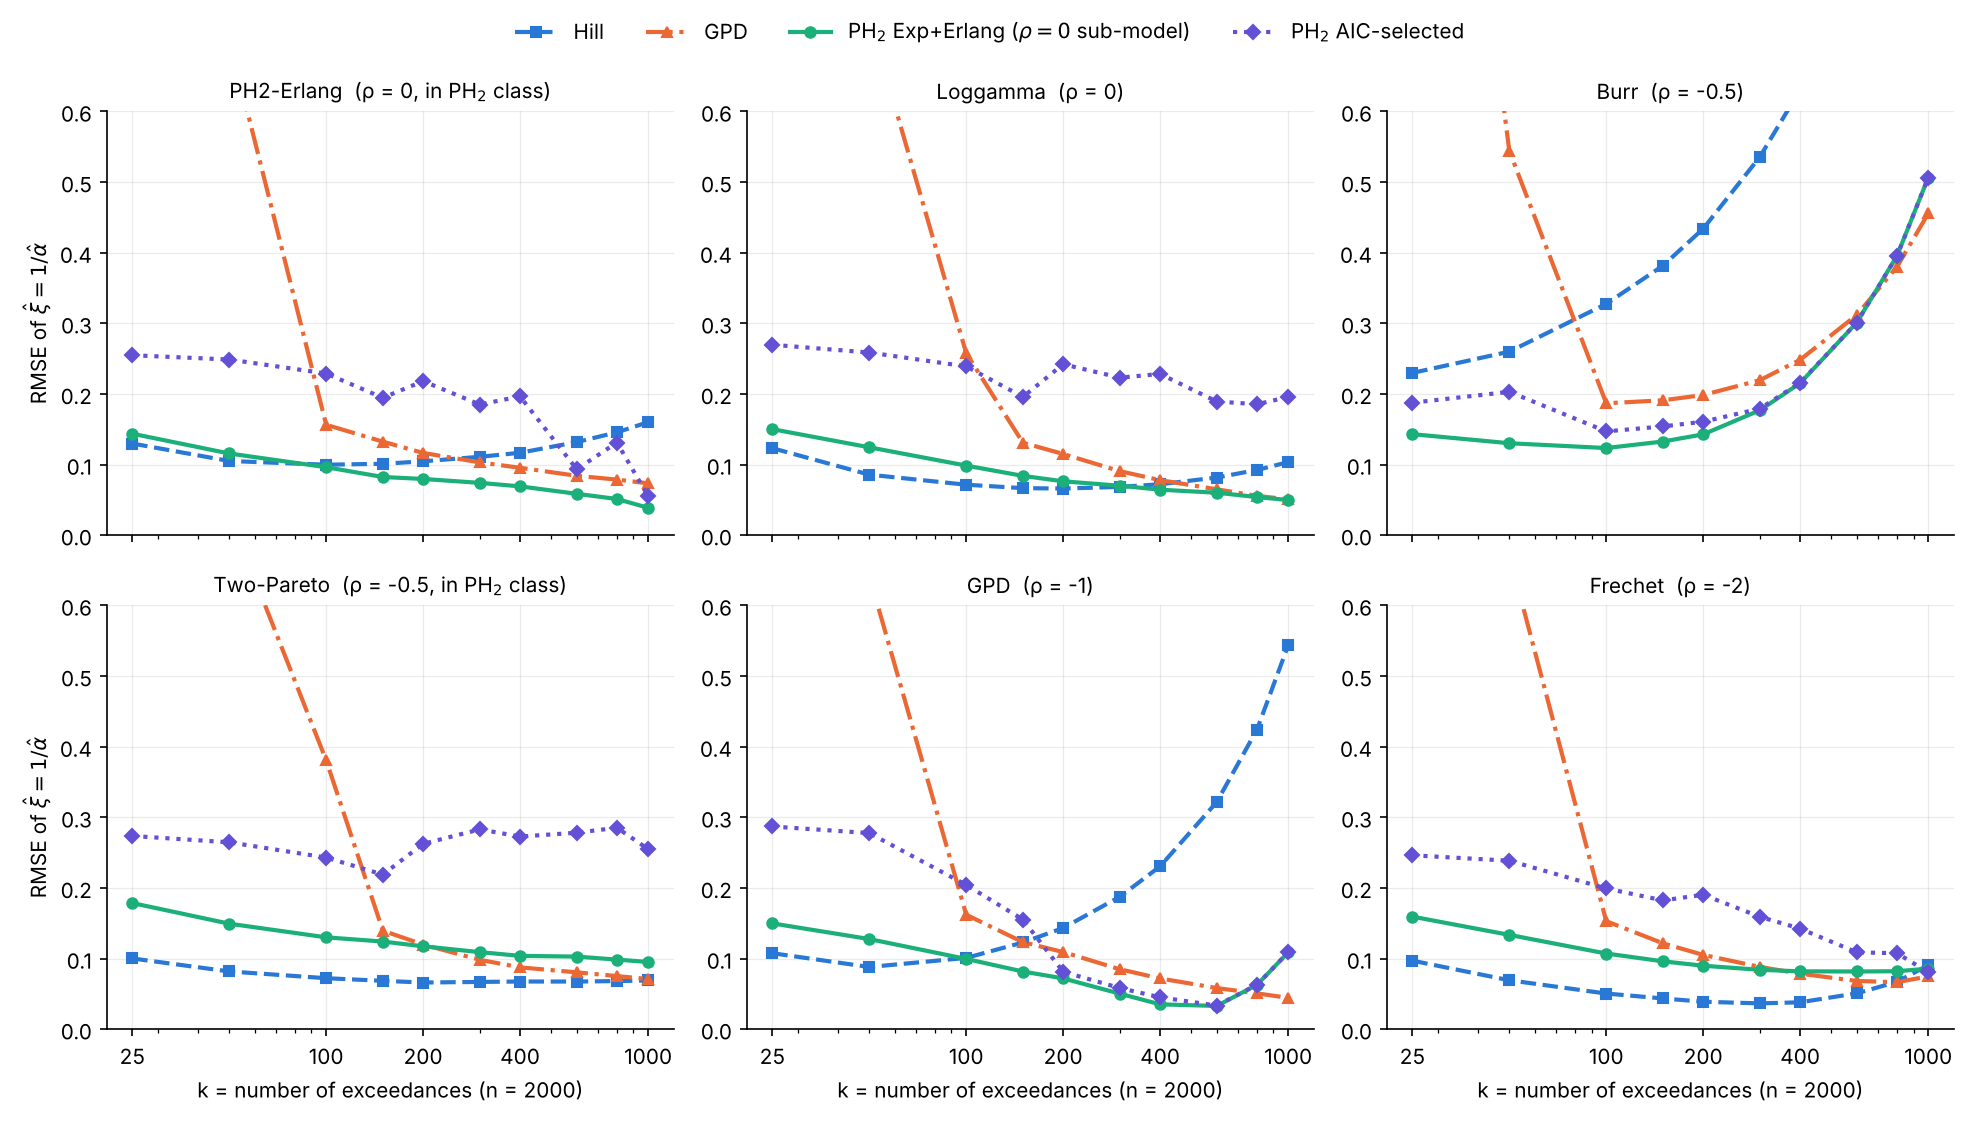
\includegraphics[width=\linewidth]{figures/rmse_xi_n2000.png}
\caption{RMSE of $\hat\xi$ against the number of exceedances $k$ (log scale), $n=2000$, $R=500$.}
\label{fig:rmse2000}
\end{figure}

\begin{figure}[t]
\centering
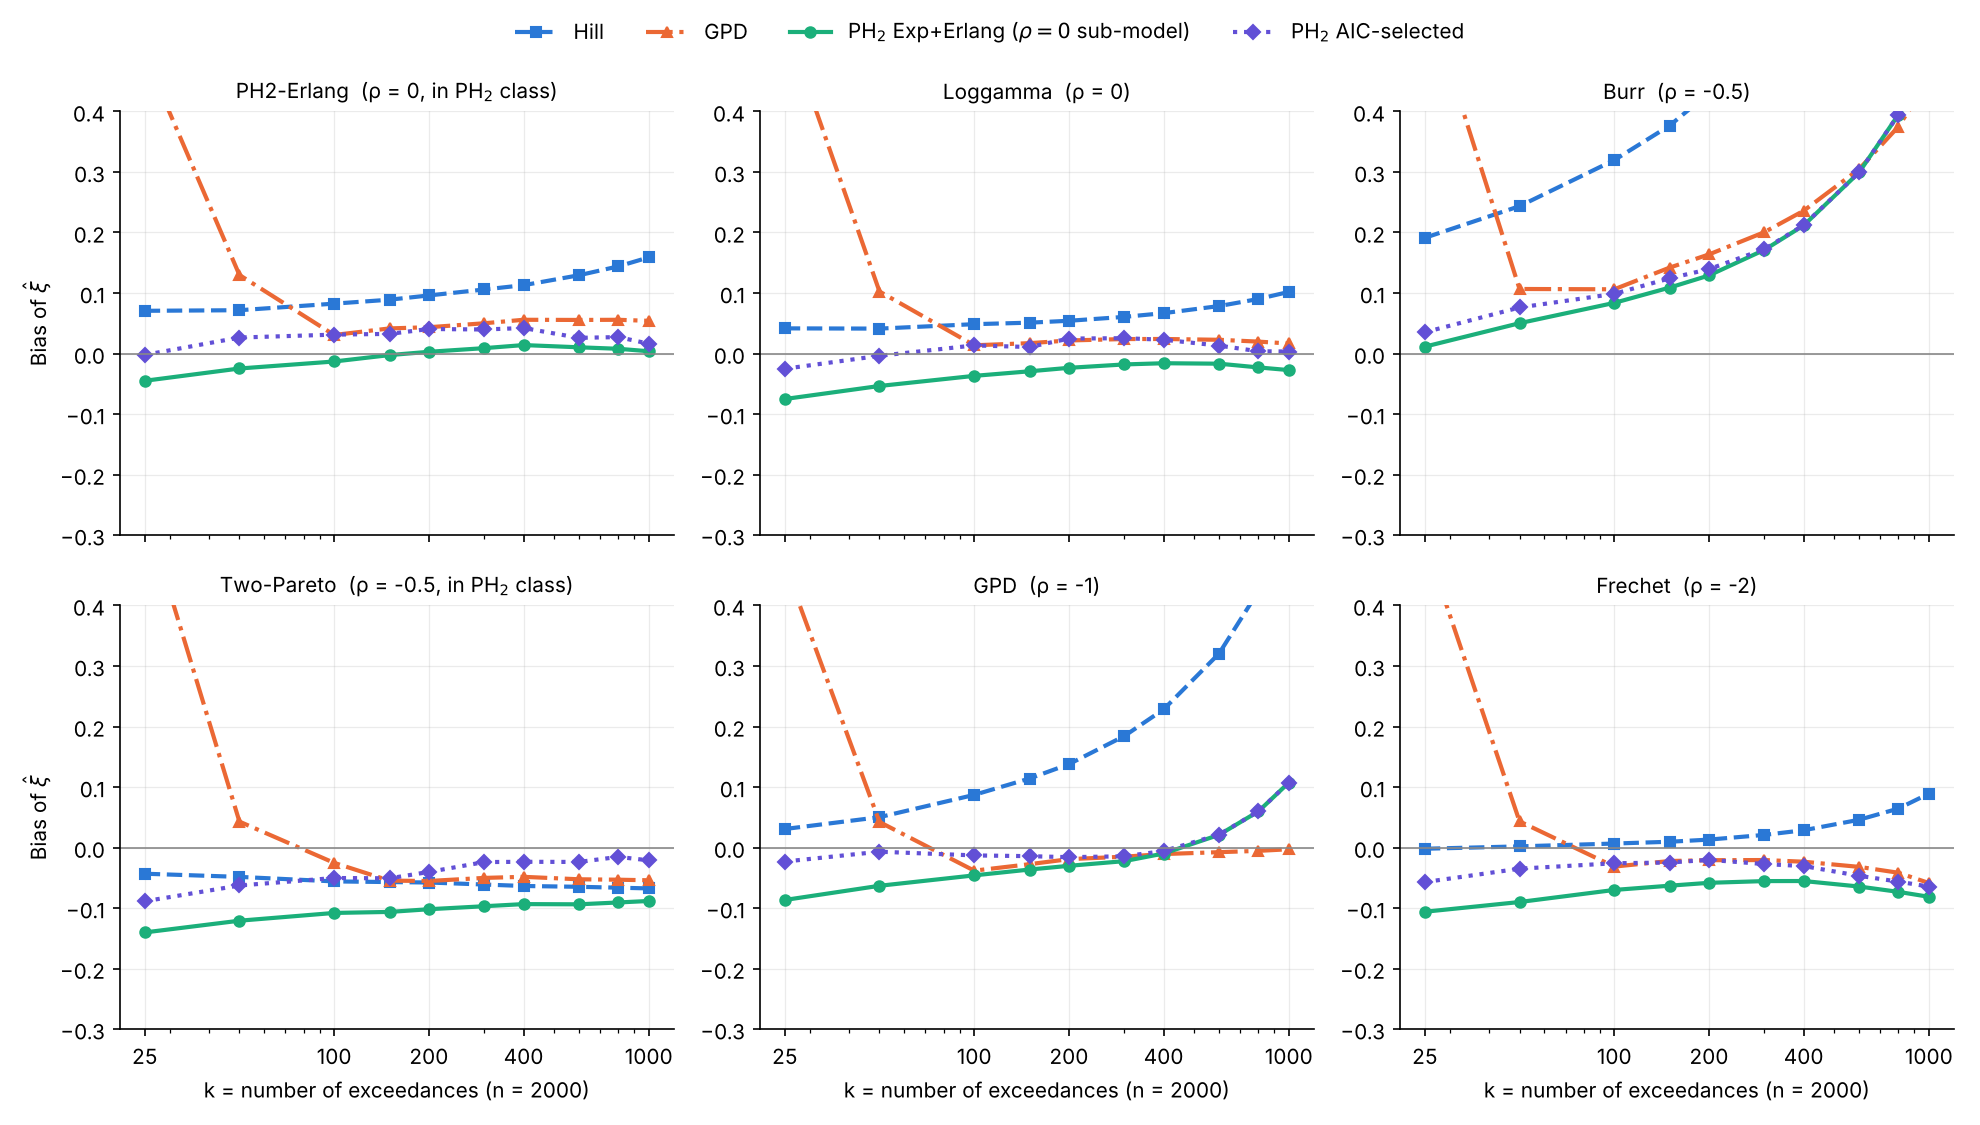
\includegraphics[width=\linewidth]{figures/bias_xi_n2000.png}
\caption{Bias of $\hat\xi$ against $k$, $n=2000$, $R=500$.}
\label{fig:bias2000}
\end{figure}

\subsection{High quantiles}\label{sec:simq}

Table~\ref{tab:q2000} and Figure~\ref{fig:q2000} report the accuracy of $\widehat{\VaR}_{0.9995}$ for $n=2000$. The differences are smaller than for $\hat\xi$, since all methods estimate the quantile from the same exceedances. E+E has a lower quantile RMSE than GPD at every $k\le400$ for five of the six DGPs; for Burr it does so only up to $k=200$ (see \texttt{sim/summary\_by\_k.csv}). The Weissman--Hill quantile is best for the near-Pareto Two-Pareto and Fr\'echet tails at moderate $k$, but it deteriorates sharply at large $k$ under GPD and Burr tails. Under the GPD and Burr DGPs all log-scale methods, E+E included, deteriorate once $k$ exceeds roughly 15--30\% of the sample: there $\log(Y/u)$ is dominated by observations near zero, outside the tail regime. The GPD fit on the original scale is unaffected by this.

\begin{table}[t]
\centering
\footnotesize
\setlength{\tabcolsep}{4pt}
\caption{RMSE of $\log(\widehat{\mathrm{VaR}}_{0.9995}/\mathrm{VaR}_{0.9995})$ over $k\in\{50,\dots,1000\}$, $n=2000$, $R=500$.}
\label{tab:q2000}
\begin{tabular}{llrrrrrrrr}
\toprule
 & & \multicolumn{4}{c}{Best $k$} & \multicolumn{4}{c}{Worst $k$} \\
\cmidrule(lr){3-6} \cmidrule(lr){7-10}
DGP & $\rho$ & Hill & GPD & E+E & AIC & Hill & GPD & E+E & AIC \\
\midrule
PH$_2$-Erlang & $0$ & 0.251 & 0.229 & \textbf{0.197} & 0.211 & 0.473 & 0.434 & \textbf{0.347} & 0.379 \\
Loggamma & $0$ & 0.204 & 0.220 & \textbf{0.194} & 0.229 & \textbf{0.339} & 0.446 & 0.348 & 0.385 \\
Burr & $-0.5$ & 0.429 & 0.388 & \textbf{0.327} & 0.351 & 3.000 & \textbf{1.193} & 2.228 & 2.228 \\
Two-Pareto & $-0.5$ & \textbf{0.137} & 0.201 & 0.189 & 0.281 & \textbf{0.268} & 0.363 & 0.294 & 0.334 \\
GPD & $-1$ & 0.286 & \textbf{0.197} & 0.220 & 0.233 & 2.551 & \textbf{0.402} & 0.761 & 0.761 \\
Fr\'echet & $-2$ & \textbf{0.187} & 0.237 & 0.189 & 0.190 & 0.465 & 0.393 & \textbf{0.320} & 0.357 \\
\bottomrule
\end{tabular}
\par\smallskip
\parbox{\linewidth}{\footnotesize Log-ratio errors are truncated at $\pm 3$ before averaging. ``Best'' is the smallest RMSE over the threshold grid (oracle threshold); ``worst'' is the largest RMSE over the grid, a measure of sensitivity to the threshold choice. The smallest value in each row and block is in bold.}
\end{table}


\begin{figure}[t]
\centering
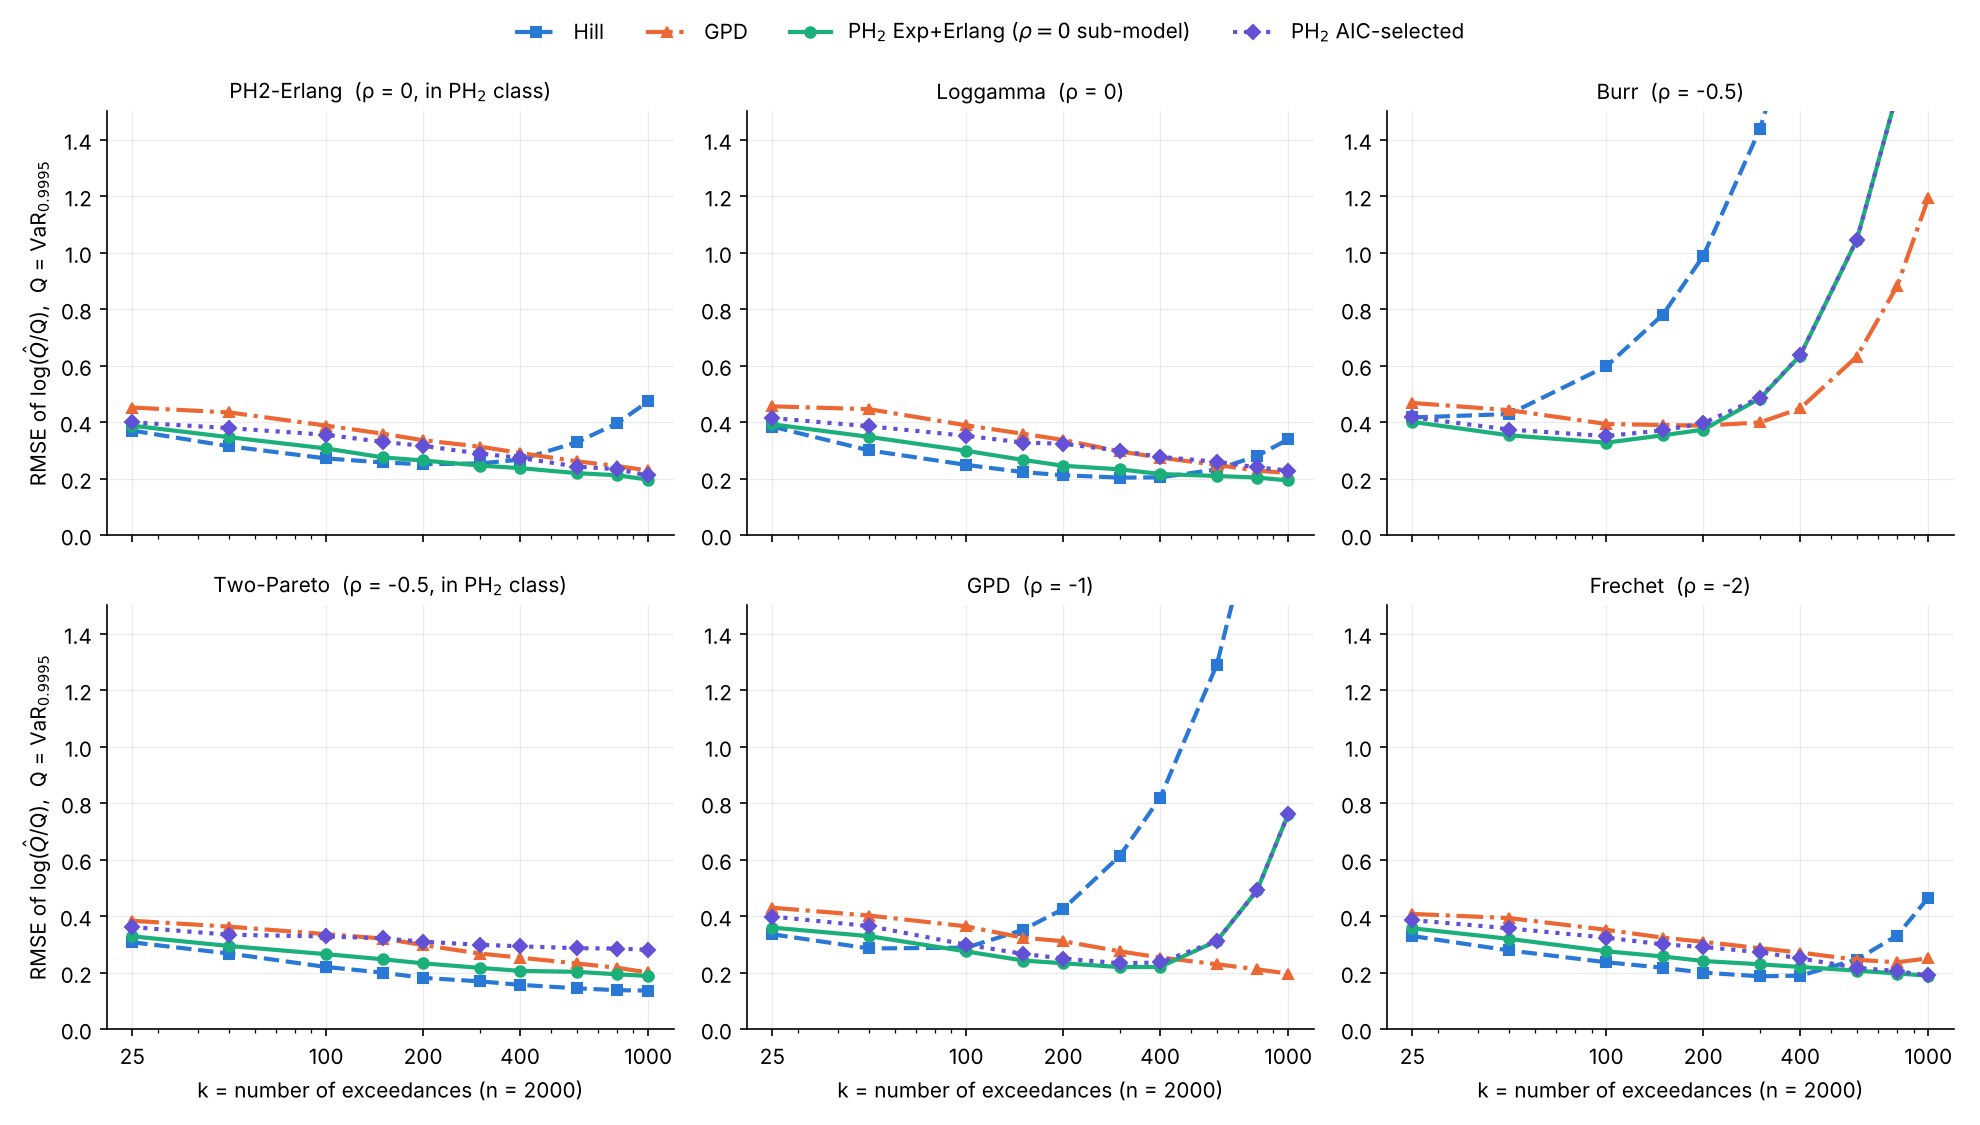
\includegraphics[width=\linewidth]{figures/rmse_q_n2000.png}
\caption{RMSE of $\log(\widehat{\VaR}_{0.9995}/\VaR_{0.9995})$ against $k$, $n=2000$, $R=500$.}
\label{fig:q2000}
\end{figure}

\subsection{Identification of the second-order case}\label{sec:rhoid}

A natural hope is that the fitted PH$_2$ sub-family indicates which second-order case the data are in: EE for $\rho=0$ and 2E for $\rho<0$. The evidence does not support this. Table~\ref{tab:share} shows that AIC selects EE in at least half, and usually 70--100\%, of the samples for every DGP, including those with $\rho=-0.5$, $-1$ and $-2$, while BIC selects EE in more than 90\% of samples. Increasing $n$ from 2000 to 10\,000 does not change the picture. The only DGP for which selection moves decisively to 2E is the GPD with location 5 fitted without the shift; there the second exponential absorbs the support offset, not a second-order term.

Table~\ref{tab:cond} shows that selecting 2E is also harmful for estimation. When AIC selects 2E, the RMSE of $\hat\xi$ is typically several times larger than when it selects EE, even for the in-class Two-Pareto DGP; the only exception is the Fr\'echet DGP at the largest threshold. The implied $\hat\rho=-\hat\tau$ ranges from about $-2$ to $-33$, regardless of whether the true $\rho$ is $0$, $-0.5$, $-1$ or $-2$. In these fits the faster exponential describes the shape of the log-excess just above the threshold rather than a second-order tail term. These findings agree with the non-regularity described in Section~\ref{sec:selection}.

\begin{table}[t]
\centering
\footnotesize
\setlength{\tabcolsep}{4pt}
\caption{Proportion of samples in which the $\rho=0$ (Exp+Erlang) sub-family is selected over the two-exponential sub-family ($\rho<0$).}
\label{tab:share}
\begin{tabular}{llrrrrrrrrrrrr}
\toprule
 & & \multicolumn{6}{c}{$n=2000$, $k=$} & \multicolumn{6}{c}{$n=10\,000$, $k=$} \\
\cmidrule(lr){3-8} \cmidrule(lr){9-14}
 & & \multicolumn{3}{c}{AIC} & \multicolumn{3}{c}{BIC} & \multicolumn{3}{c}{AIC} & \multicolumn{3}{c}{BIC} \\
\cmidrule(lr){3-5} \cmidrule(lr){6-8} \cmidrule(lr){9-11} \cmidrule(lr){12-14}
DGP & $\rho$ & 100 & 400 & 1000 & 100 & 400 & 1000 & 500 & 2000 & 5000 & 500 & 2000 & 5000 \\
\midrule
PH$_2$-Erlang & $0$ & 0.79 & 0.84 & 0.89 & 0.97 & 0.98 & 0.99 & 0.78 & 0.88 & 0.92 & 0.99 & 1.00 & 1.00 \\
Loggamma & $0$ & 0.76 & 0.79 & 0.83 & 0.95 & 0.98 & 1.00 & 0.75 & 0.82 & 0.87 & 0.98 & 0.99 & 1.00 \\
Burr & $-0.5$ & 0.90 & 1.00 & 1.00 & 0.98 & 1.00 & 1.00 & 0.97 & 1.00 & 1.00 & 1.00 & 1.00 & 1.00 \\
Two-Pareto & $-0.5$ & 0.72 & 0.62 & 0.61 & 0.94 & 0.94 & 0.97 & 0.60 & 0.60 & 0.50 & 0.95 & 0.96 & 0.96 \\
GPD & $-1$ & 0.83 & 0.98 & 1.00 & 0.97 & 1.00 & 1.00 & 0.87 & 0.99 & 1.00 & 0.99 & 1.00 & 1.00 \\
GPD, $\mu=5$ & $-1$ & -- & -- & -- & -- & -- & -- & 0.30 & 0.00 & 0.00 & 0.78 & 0.01 & 0.00 \\
Fr\'echet & $-2$ & 0.74 & 0.79 & 0.85 & 0.96 & 0.98 & 0.99 & 0.71 & 0.82 & 0.67 & 0.96 & 0.99 & 0.97 \\
\bottomrule
\end{tabular}
\par\smallskip
\parbox{\linewidth}{\footnotesize The GPD with location $\mu=5$ was included only in the $n=10\,000$ study. Fits are on the unshifted log-excesses.}
\end{table}

\begin{table}[t]
\centering
\small
\caption{RMSE of $\hat\xi$ for the AIC-selected PH$_2$ fit, split by the selected sub-family, and median $\hat\rho=-\hat\tau$ among fits selecting the two-exponential sub-family.}
\label{tab:cond}
\begin{tabular}{rlrrrrrr}
\toprule
$n$ & DGP ($\rho$) & $k$ & \#$\rho<0$ & \#$\rho=0$ & RMSE, $\rho<0$ & RMSE, $\rho=0$ & median $\hat\rho$ \\
\midrule
2000 & PH$_2$-Erlang ($0$) & 400 & 78 & 422 & 0.473 & 0.067 & -32.72 \\
 & PH$_2$-Erlang ($0$) & 1000 & 53 & 447 & 0.131 & 0.037 & -10.61 \\
 & Loggamma ($0$) & 400 & 104 & 396 & 0.484 & 0.065 & -26.35 \\
 & Loggamma ($0$) & 1000 & 84 & 416 & 0.465 & 0.049 & -9.27 \\
 & Burr ($-0.5$) & 400 & 1 & 499 & 0.388 & 0.215 & -4.24 \\
 & Burr ($-0.5$) & 1000 & -- & 500 & -- & 0.506 & -- \\
 & Two-Pareto ($-0.5$) & 400 & 191 & 309 & 0.418 & 0.112 & -14.03 \\
 & Two-Pareto ($-0.5$) & 1000 & 194 & 306 & 0.388 & 0.103 & -8.64 \\
 & GPD ($-1$) & 400 & 12 & 488 & 0.188 & 0.035 & -13.22 \\
 & GPD ($-1$) & 1000 & -- & 500 & -- & 0.109 & -- \\
 & Fr\'echet ($-2$) & 400 & 104 & 396 & 0.265 & 0.085 & -29.95 \\
 & Fr\'echet ($-2$) & 1000 & 74 & 426 & 0.041 & 0.086 & -4.85 \\
\midrule
10000 & PH$_2$-Erlang ($0$) & 2000 & 60 & 440 & 0.456 & 0.038 & -21.57 \\
 & PH$_2$-Erlang ($0$) & 5000 & 42 & 458 & 0.113 & 0.016 & -2.82 \\
 & Loggamma ($0$) & 2000 & 90 & 410 & 0.543 & 0.043 & -20.83 \\
 & Loggamma ($0$) & 5000 & 67 & 433 & 0.066 & 0.035 & -3.20 \\
 & Burr ($-0.5$) & 2000 & -- & 500 & -- & 0.214 & -- \\
 & Burr ($-0.5$) & 5000 & -- & 500 & -- & 0.504 & -- \\
 & Two-Pareto ($-0.5$) & 2000 & 200 & 300 & 0.274 & 0.088 & -3.90 \\
 & Two-Pareto ($-0.5$) & 5000 & 249 & 251 & 0.254 & 0.083 & -2.33 \\
 & GPD ($-1$) & 2000 & 4 & 496 & 0.120 & 0.018 & -2.06 \\
 & GPD ($-1$) & 5000 & -- & 500 & -- & 0.107 & -- \\
 & GPD, $\mu=5$ ($-1$) & 2000 & 500 & -- & 0.077 & -- & -2.69 \\
 & GPD, $\mu=5$ ($-1$) & 5000 & 500 & -- & 0.073 & -- & -3.37 \\
 & Fr\'echet ($-2$) & 2000 & 89 & 411 & 0.319 & 0.069 & -18.57 \\
 & Fr\'echet ($-2$) & 5000 & 164 & 336 & 0.020 & 0.085 & -2.31 \\
\bottomrule
\end{tabular}
\end{table}


\subsection{Larger samples and the min-shift}

Table~\ref{tab:xi10000} and Figure~\ref{fig:shift} report the study with $n=10\,000$, including the min-shifted E+E fit. The conclusions for the unshifted methods are unchanged and sharper: for the PH$_2$-Erlang DGP the best RMSE of E+E is $0.016$, against $0.062$ for GPD and $0.081$ for Hill.

The min-shift does what it is designed for and no more. For the GPD with location 5, the unshifted Hill and E+E fits have a bias of about $-0.2$ at large $k$, while E+E$_s$ attains RMSE $0.019$, comparable to the GPD fit ($0.021$). For DGPs supported on $[0,\infty)$ (GPD, Burr) the shift has no visible effect, so it does not cure the large-$k$ breakdown noted above. For DGPs supported on $[1,\infty)$ the shift distorts the fit at large $k$, since $\log(Y-1)$ is no longer PH$_2$; the small best-$k$ RMSE of E+E$_s$ for Loggamma and Two-Pareto in Table~\ref{tab:xi10000} occurs where its bias changes sign and does not reflect a uniform improvement. The shift should therefore be applied only when there is evidence that the support starts away from zero, as recommended by \citet{KimKim2015}.

\begin{table}[t]
\centering
\small
\caption{RMSE of $\hat\xi$ over $k\in\{250,\dots,5000\}$, $n=10\,000$, $R=500$.}
\label{tab:xi10000}
\begin{tabular}{llrrrrrrrrrr}
\toprule
 & & \multicolumn{5}{c}{Best $k$} & \multicolumn{5}{c}{Worst $k$} \\
\cmidrule(lr){3-7} \cmidrule(lr){8-12}
DGP & $\rho$ & Hill & GPD & E+E & E+E$_s$ & AIC & Hill & GPD & E+E & E+E$_s$ & AIC \\
\midrule
PH$_2$-Erlang & $0$ & 0.081 & 0.062 & \textbf{0.016} & 0.027 & 0.035 & 0.160 & 0.105 & \textbf{0.072} & 0.124 & 0.231 \\
Loggamma & $0$ & 0.054 & 0.028 & 0.034 & \textbf{0.017} & 0.040 & 0.104 & 0.100 & \textbf{0.075} & 0.081 & 0.259 \\
Burr & $-0.5$ & 0.242 & 0.132 & \textbf{0.086} & \textbf{0.086} & 0.097 & 1.282 & \textbf{0.454} & 0.504 & 0.504 & 0.504 \\
Two-Pareto & $-0.5$ & 0.058 & 0.057 & 0.078 & \textbf{0.013} & 0.157 & \textbf{0.067} & 0.105 & 0.108 & 0.098 & 0.206 \\
GPD & $-1$ & 0.067 & 0.020 & \textbf{0.018} & \textbf{0.018} & 0.021 & 0.542 & \textbf{0.099} & 0.107 & 0.107 & 0.184 \\
GPD, $\mu=5$ & $-1$ & 0.074 & 0.021 & 0.096 & \textbf{0.019} & 0.065 & 0.200 & \textbf{0.095} & 0.200 & 0.106 & 0.219 \\
Fr\'echet & $-2$ & \textbf{0.021} & 0.038 & 0.064 & 0.043 & 0.067 & 0.089 & 0.099 & 0.085 & \textbf{0.084} & 0.258 \\
\bottomrule
\end{tabular}
\par\smallskip
\parbox{\linewidth}{\footnotesize E+E$_s$: Exp+Erlang sub-model fitted to the min-shifted log-excesses $\log\{(Y-m)/(u-m)\}$, $m=\min_i Y_i$. For Loggamma and Two-Pareto the small best-$k$ value of E+E$_s$ occurs where its bias changes sign and should not be read as a uniform advantage. E+E: PH$_2$ Exp+Erlang ($\rho=0$) sub-model; AIC: PH$_2$ with the sub-family chosen by AIC. ``Best'' is the smallest RMSE over the threshold grid (oracle threshold); ``worst'' is the largest RMSE over the grid, a measure of sensitivity to the threshold choice. The smallest value in each row and block is in bold.}
\end{table}


\begin{figure}[t]
\centering
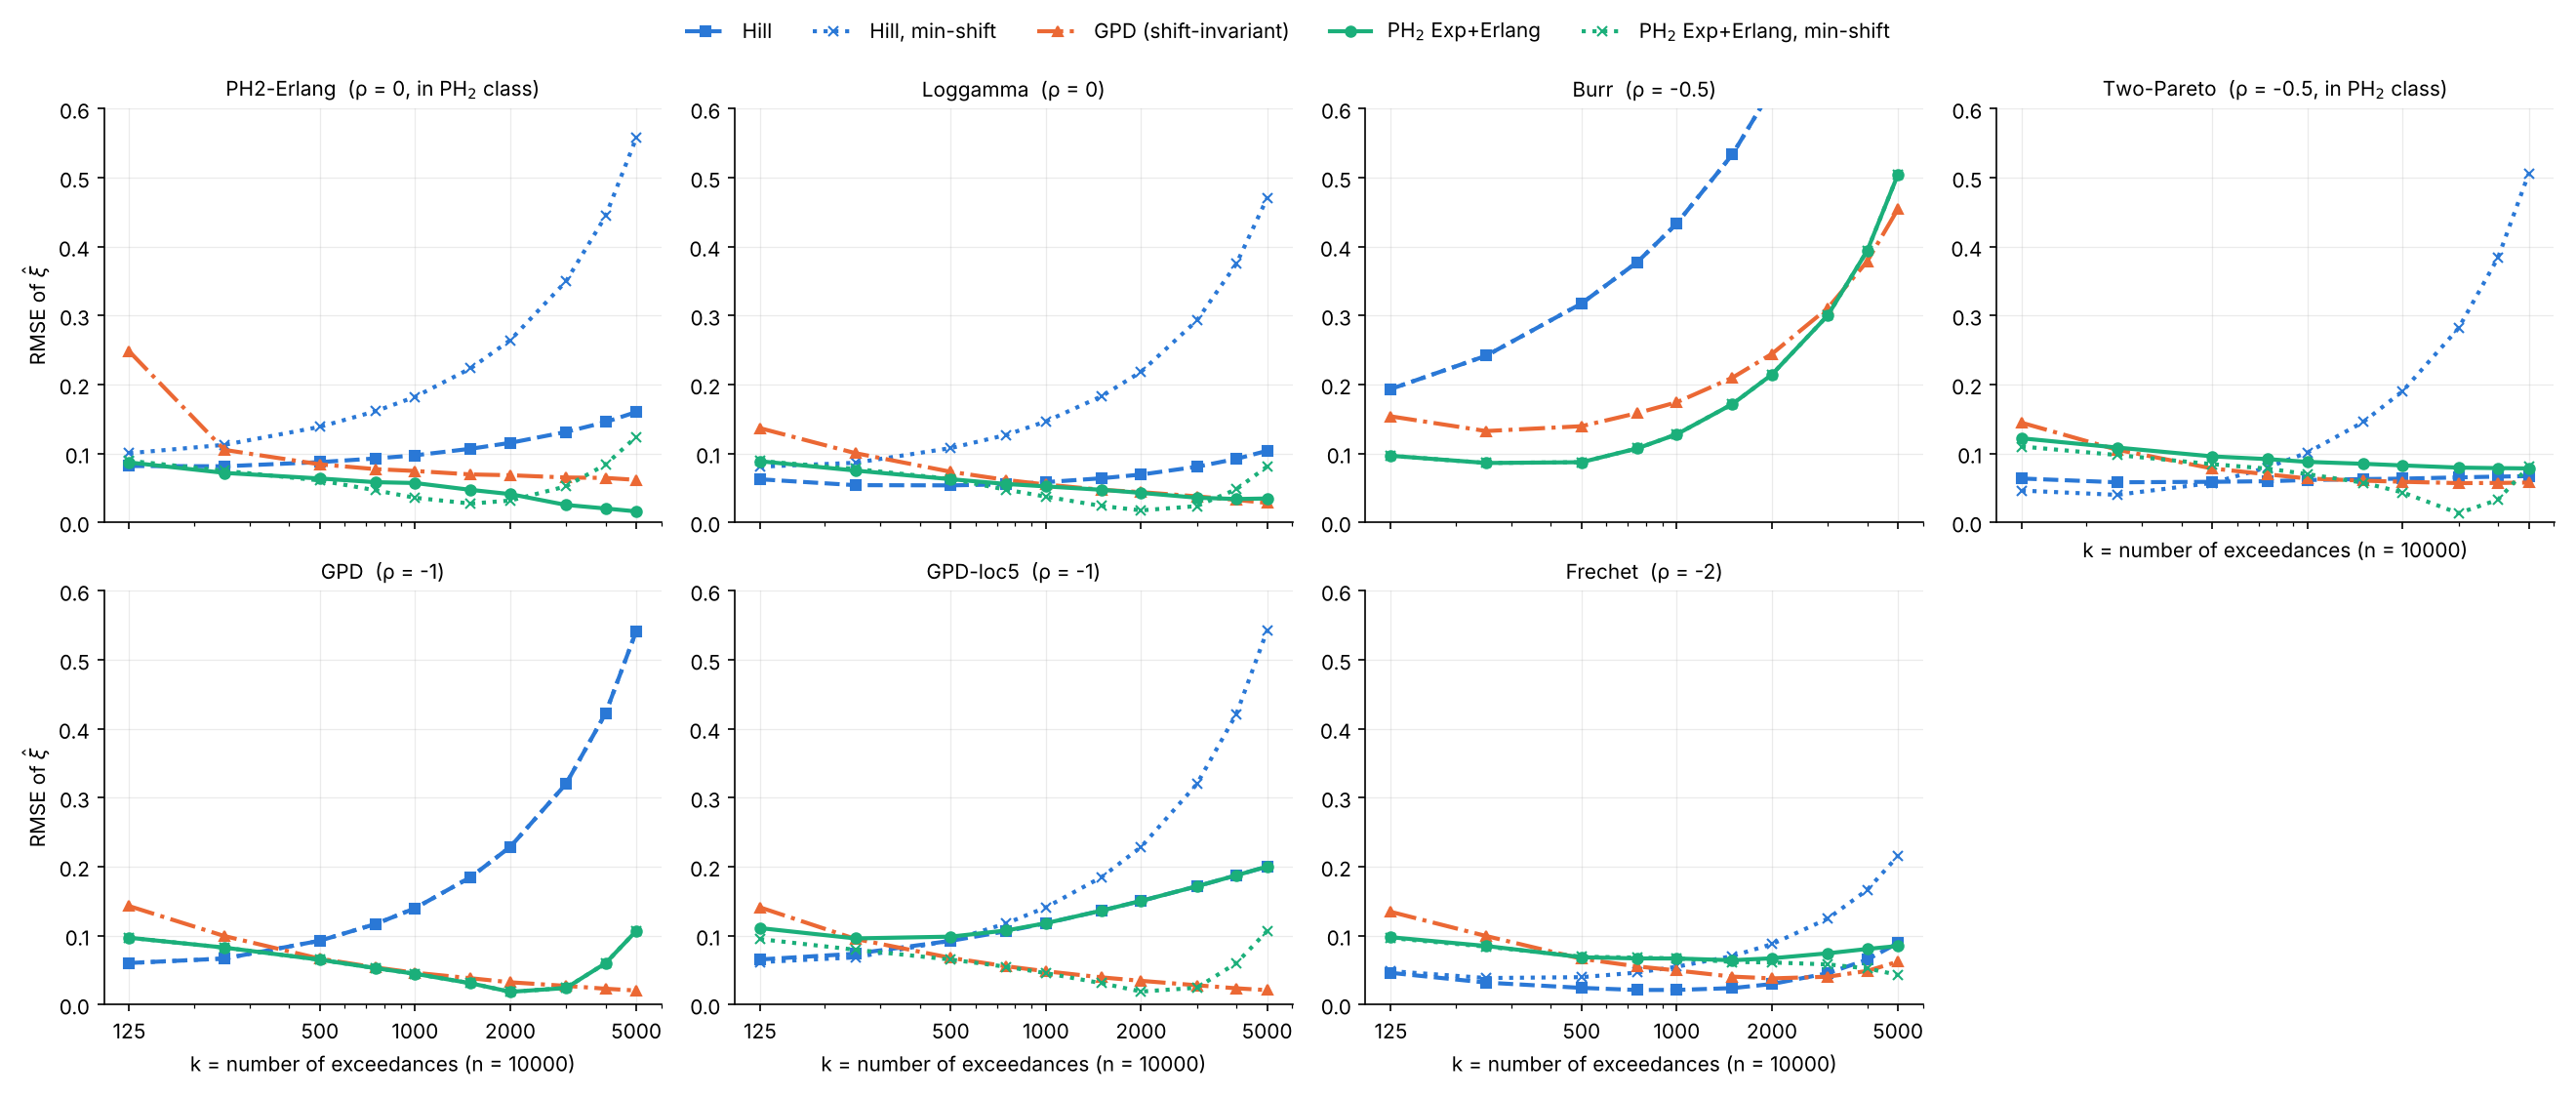
\includegraphics[width=\linewidth]{figures/shift_rmse_xi_n10000.png}
\caption{RMSE of $\hat\xi$ against $k$ for $n=10\,000$, with and without the min-shift. For GPD and Burr the shifted and unshifted curves coincide.}
\label{fig:shift}
\end{figure}

\subsection{Coverage of interval estimates}\label{sec:coverage}

Table~\ref{tab:cov} reports the coverage of nominal 95\% intervals for $\xi$ when $n=2000$. Where the E+E fit is approximately unbiased, the profile-likelihood interval \eqref{eq:profile} attains close to nominal coverage: $0.92$--$0.97$ under the in-class PH$_2$-Erlang DGP, $0.88$--$0.96$ under Loggamma, and $0.93$--$0.96$ under the GPD for $k\le500$. Wald intervals based on \eqref{eq:fisher} are unreliable, because $\hat p$ is close to zero in a substantial fraction of samples (last column), where the interval becomes uninformative. The Hill interval $\hat\xi^H\pm1.96\,\hat\xi^H/\sqrt k$ under-covers in every setting, often severely, because its bias is large relative to its standard error. No interval can correct a biased point estimate: under the Two-Pareto DGP, where E+E has a bias of about $-0.09$, and under the GPD at $k=1000$, where the log-scale fit breaks down, the profile interval also fails. Interval estimates are therefore only as reliable as the threshold region from which they are taken, which reinforces recommendation~1 in Section~\ref{sec:discussion}.

\IfFileExists{tables/tab_cov.tex}{\begin{table}[t]
\centering
\footnotesize
\setlength{\tabcolsep}{4pt}
\caption{Empirical coverage (mean width) of nominal 95\% intervals for $\xi=0.5$, $n=2000$, $R=500$.}
\label{tab:cov}
\begin{tabular}{lrlllr}
\toprule
DGP & $k$ & Wald, E+E & Profile, E+E & Hill & $\Pr(\hat p<0.01)$ \\
\midrule
PH$_2$-Erlang & 200 & 0.896 (3.042) & 0.966 (0.287) & 0.378 (0.165) & 0.27 \\
 & 500 & 0.920 (1.704) & 0.962 (0.227) & 0.004 (0.109) & 0.15 \\
 & 1000 & 0.940 (0.368) & 0.924 (0.164) & 0.000 (0.082) & 0.02 \\
\midrule
Loggamma & 200 & 0.842 (3.466) & 0.964 (0.267) & 0.776 (0.153) & 0.31 \\
 & 500 & 0.850 (2.400) & 0.938 (0.212) & 0.156 (0.101) & 0.22 \\
 & 1000 & 0.756 (0.567) & 0.878 (0.166) & 0.000 (0.075) & 0.04 \\
\midrule
Two-Pareto & 200 & 0.760 (5.510) & 0.520 (0.206) & 0.498 (0.122) & 0.53 \\
 & 500 & 0.714 (5.521) & 0.126 (0.154) & 0.106 (0.076) & 0.54 \\
 & 1000 & 0.744 (6.119) & 0.008 (0.123) & 0.006 (0.054) & 0.61 \\
\midrule
GPD & 200 & 0.816 (1.070) & 0.930 (0.286) & 0.092 (0.177) & 0.08 \\
 & 500 & 0.976 (0.129) & 0.964 (0.136) & 0.000 (0.135) & 0.00 \\
 & 1000 & 0.000 (0.082) & 0.000 (0.080) & 0.000 (0.129) & 0.00 \\
\bottomrule
\end{tabular}
\par\smallskip
\parbox{\linewidth}{\footnotesize Wald intervals whose width exceeds 10, or whose estimated information is numerically singular (near $\hat p=0$), are treated as uninformative: width 10, counted as covering. Last column: proportion of fits with $\hat p<0.01$.}
\end{table}
}{\todo{Coverage table pending: run \texttt{sim/fisher\_B.py coverage} and \texttt{make\_tables.py}.}}

\subsection{Coverage of interval estimates for risk measures}\label{sec:coveragerisk}

Table~\ref{tab:covrisk} reports the coverage of the 95\% profile-likelihood intervals of Section~\ref{sec:riskci} for $\VaR_{0.995}$ and $\mathrm{ES}_{0.995}$, for $n=2000$, $R=300$ and three DGPs. The true expected shortfall is computed from the true survival function. For PH$_2$-Erlang this is the closed form \eqref{eq:es} with $u=1$; for Loggamma it requires numerical integration. The E+E intervals attain coverage between $0.92$ and $0.97$ in eleven of the twelve settings. The exception is the GPD DGP at $k=500$ ($0.857$ for expected shortfall), where the log-scale fit is entering the region in which it breaks down (Section~\ref{sec:simq}). The GPD intervals also have close to nominal coverage, between $0.92$ and $0.96$. For expected shortfall, however, their median width is considerably larger than that of the E+E intervals: $140$ against $75$ under PH$_2$-Erlang at $k=200$, and $102$ against $52$ under Loggamma. The intervals based on the Pareto (Hill) tail are short but increasingly biased as $k$ grows. Their coverage for expected shortfall falls to $0.66$ under PH$_2$-Erlang and to zero under the GPD DGP at $k=500$. Under the conditions for which it was designed, the E+E tail therefore delivers risk-measure intervals that are both close to nominal and substantially shorter than the GPD intervals, especially for expected shortfall, which depends most on the extrapolation.

\IfFileExists{tables/tab_cov_risk.tex}{\begin{table}[t]
\centering
\footnotesize
\setlength{\tabcolsep}{4pt}
\caption{Empirical coverage (median width) of 95\% profile-likelihood intervals for $\mathrm{VaR}_{0.995}$ and $\mathrm{ES}_{0.995}$, $n=2000$, $R=300$.}
\label{tab:covrisk}
\begin{tabular}{lrlrlll}
\toprule
DGP & $k$ & Measure & True value & Hill & GPD & E+E \\
\midrule
PH$_2$-Erlang & 200 & $\mathrm{VaR}_{0.995}$ & 29.63 & 0.910 (15.5) & 0.937 (17.8) & 0.933 (15.3) \\
 & 200 & $\mathrm{ES}_{0.995}$ & 66.00 & 0.873 (74.1) & 0.953 (139.9) & 0.950 (75.0) \\
 & 500 & $\mathrm{VaR}_{0.995}$ & 29.63 & 0.850 (14.1) & 0.950 (16.3) & 0.960 (14.8) \\
 & 500 & $\mathrm{ES}_{0.995}$ & 66.00 & 0.657 (64.7) & 0.960 (86.8) & 0.967 (66.9) \\
\midrule
Loggamma & 200 & $\mathrm{VaR}_{0.995}$ & 24.77 & 0.937 (12.3) & 0.927 (14.2) & 0.920 (12.1) \\
 & 200 & $\mathrm{ES}_{0.995}$ & 52.56 & 0.930 (52.7) & 0.923 (101.5) & 0.947 (52.0) \\
 & 500 & $\mathrm{VaR}_{0.995}$ & 24.77 & 0.890 (10.7) & 0.940 (13.7) & 0.953 (11.6) \\
 & 500 & $\mathrm{ES}_{0.995}$ & 52.56 & 0.787 (42.0) & 0.937 (68.1) & 0.963 (46.5) \\
\midrule
GPD & 200 & $\mathrm{VaR}_{0.995}$ & 26.28 & 0.873 (16.5) & 0.940 (14.3) & 0.950 (14.1) \\
 & 200 & $\mathrm{ES}_{0.995}$ & 54.57 & 0.557 (99.4) & 0.950 (82.2) & 0.950 (69.4) \\
 & 500 & $\mathrm{VaR}_{0.995}$ & 26.28 & 0.037 (22.5) & 0.940 (14.3) & 0.917 (13.9) \\
 & 500 & $\mathrm{ES}_{0.995}$ & 54.57 & 0.000 (248.6) & 0.940 (63.1) & 0.857 (56.2) \\
\bottomrule
\end{tabular}
\end{table}
}{}

\section{Empirical illustration}\label{sec:data}

We apply the methods to the Danish fire insurance losses analysed by \citet{McNeil1997} and \citet{Resnick1997}, among others: $n=2167$ losses from 1980--1990, in millions of Danish kroner. All losses exceed one million kroner, so the data are left-truncated at $1$. As the support of the underlying loss starts at zero, we follow \citet{KimKim2015} and do not apply the min-shift; all fits use the log-excesses $\log(Y/u)$. We compute the Hill, GPD and E+E estimates at 30 thresholds, with $k$ ranging from 22 to 1084 exceedances on a logarithmic grid ($u$ from about 26 down to 1.8), together with 95\% profile-likelihood intervals \eqref{eq:profile} for the E+E tail index. Figure~\ref{fig:danish} shows $\hat\xi$ and $\widehat{\VaR}_{0.995}$ against $k$. Table~\ref{tab:danish} gives the estimates at five thresholds, and Table~\ref{tab:danishsd} measures how much each estimate moves across thresholds within three windows.

Three regions can be distinguished. For the highest thresholds ($k\le56$, $u\gtrsim16$) the E+E fit returns $\hat p\approx0$ and coincides with the Hill estimator, with $\hat\xi$ between $0.52$ and $0.59$: in the extreme tail the data are consistent with an exact Pareto tail, and the profile intervals are wide, as Proposition~\ref{prop:singular} predicts near the boundary. For intermediate thresholds ($64\le k\le188$, $u\approx6$--$14$) the Erlang weight becomes substantial ($\hat p\approx0.3$--$0.7$), and the three methods diverge. The Hill estimate rises steadily from $0.58$ to $0.75$, while the E+E estimate ($0.41$--$0.50$) stays close to the GPD estimate. This is the pattern expected when the log-excesses are not exponential, so that the Hill estimator picks up second-order bias as the threshold decreases (Proposition~\ref{prop:hill}). For the lowest thresholds ($k\ge200$, $u\lesssim5.6$) all three estimates are fairly flat, but at different levels: about $0.68$--$0.73$ for Hill, $0.58$--$0.73$ for GPD and $0.55$--$0.65$ for E+E. Measured by the standard deviation of $\hat\xi$ across thresholds, E+E is the most stable estimator of the three over $50\le k\le200$ and over all thresholds together, while Hill is the flattest over $k\ge200$ (Table~\ref{tab:danishsd}). A flat Hill curve does not imply an unbiased one, however: in the simulations the Hill bias grew steadily with $k$ for the $\rho=0$ and GPD-type tails, and the Hill plateau here lies above both the GPD and the E+E estimates at 11 of these 13 thresholds, close to the upper end of the E+E profile intervals. Taking the region $k\ge200$, where the E+E and GPD estimates broadly agree, suggests $\xi\approx0.55$--$0.65$, i.e.\ $\alpha\approx1.5$--$1.8$, with a finite mean and an infinite variance.

The differences matter for risk measures. Across all thresholds, the E+E estimate of $\VaR_{0.995}$ ranges from $38.4$ to $45.3$, against $36.6$--$46.5$ for GPD and $38.4$--$50.6$ for Hill. Its standard deviation across thresholds is the smallest of the three overall and for $k\ge200$; there it is a little over half that of the GPD and under 40\% of that of the Hill estimate. For $50\le k\le200$ the GPD estimate of $\VaR_{0.995}$ is the most stable. For $\VaR_{0.999}$, which requires extrapolation beyond all but two or three observations, the E+E estimates range from $87$ to $136$, against $89$--$148$ for GPD and $88$--$170$ for Hill. All model-based estimates of $\VaR_{0.995}$ exceed the empirical $99.5\%$ quantile ($34.8$). The empirical quantile is itself based on about eleven observations, however, so this comparison cannot rank the methods.

Finally, AIC selects the EE sub-family at 29 of the 30 thresholds. The fitted 2E models give values of $\hat\tau$ ranging from essentially $0$ to several hundred. In line with Section~\ref{sec:rhoid}, we do not read either result as evidence about the second-order parameter of the Danish losses.

\begin{figure}[t]
\centering
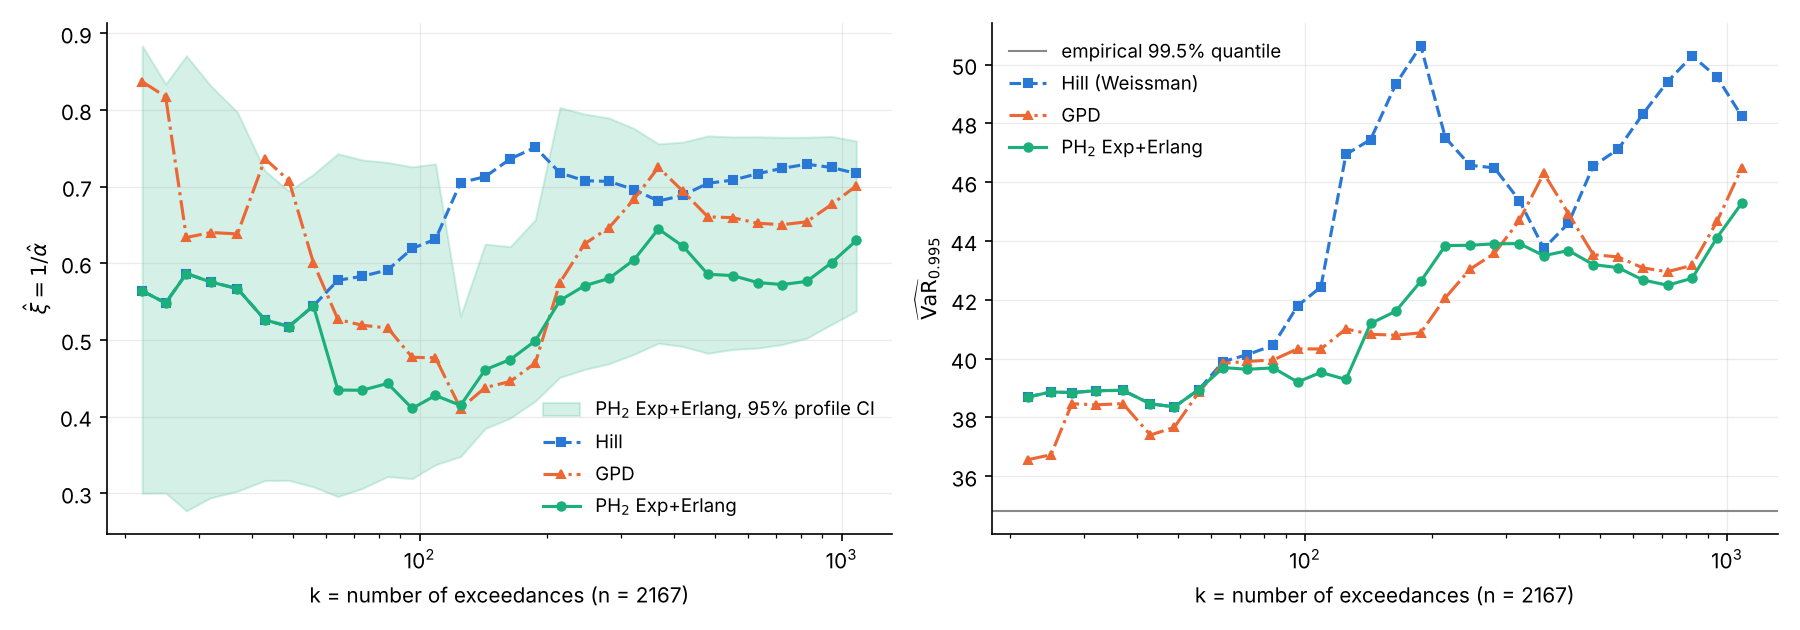
\includegraphics[width=\linewidth]{figures/danish.png}
\caption{Danish fire losses ($n=2167$). Left: $\hat\xi$ against the number of exceedances $k$ for Hill, GPD and the E+E PH$_2$ sub-model, with the 95\% profile-likelihood band for E+E. Right: the corresponding estimates of $\VaR_{0.995}$; the horizontal line is the empirical $99.5\%$ quantile.}
\label{fig:danish}
\end{figure}

\begin{table}[t]
\centering
\footnotesize
\setlength{\tabcolsep}{4pt}
\caption{Danish fire losses: tail index and VaR estimates at selected thresholds ($n=2167$, losses in millions of DKK).}
\label{tab:danish}
\begin{tabular}{rrrrlrrrrrrr}
\toprule
 & & \multicolumn{4}{c}{$\hat\xi$} & \multicolumn{3}{c}{$\widehat{\mathrm{VaR}}_{0.995}$} & \multicolumn{3}{c}{$\widehat{\mathrm{VaR}}_{0.999}$} \\
\cmidrule(lr){3-6} \cmidrule(lr){7-9} \cmidrule(lr){10-12}
$k$ & $u$ & Hill & GPD & E+E (95\% profile CI) & $\hat p$ & Hill & GPD & E+E & Hill & GPD & E+E \\
\midrule
56 & 15.93 & 0.544 & 0.601 & 0.544 (0.308, 0.716) & 0.00 & 38.9 & 38.9 & 38.9 & 93.5 & 98.4 & 93.6 \\
109 & 9.88 & 0.631 & 0.477 & 0.428 (0.337, 0.730) & 0.48 & 42.4 & 40.3 & 39.5 & 117.2 & 93.0 & 89.7 \\
246 & 5.11 & 0.708 & 0.625 & 0.571 (0.461, 0.795) & 0.24 & 46.6 & 43.0 & 43.9 & 145.5 & 119.8 & 123.6 \\
482 & 3.21 & 0.704 & 0.660 & 0.586 (0.483, 0.766) & 0.20 & 46.6 & 43.5 & 43.2 & 144.6 & 126.7 & 122.8 \\
1084 & 1.77 & 0.717 & 0.701 & 0.630 (0.538, 0.759) & 0.14 & 48.2 & 46.5 & 45.3 & 153.0 & 143.8 & 135.6 \\
\bottomrule
\end{tabular}
\par\smallskip
\parbox{\linewidth}{\footnotesize Empirical quantiles: 99.5\%: 34.8; 99.9\%: 131.6. $\hat p$ is the fitted Erlang weight of the E+E model; $\hat p\approx 0$ means that E+E coincides with the Hill estimator.}
\end{table}

\begin{table}[t]
\centering
\footnotesize
\setlength{\tabcolsep}{4pt}
\caption{Danish fire losses: standard deviation of each estimate across the thresholds of Figure~\ref{fig:danish} within three threshold windows (smallest value in bold).}
\label{tab:danishsd}
\begin{tabular}{lrrrrrrrrr}
\toprule
 & \multicolumn{3}{c}{$\hat\xi$} & \multicolumn{3}{c}{$\widehat{\mathrm{VaR}}_{0.995}$} & \multicolumn{3}{c}{$\widehat{\mathrm{VaR}}_{0.999}$} \\
\cmidrule(lr){2-4} \cmidrule(lr){5-7} \cmidrule(lr){8-10}
Window & Hill & GPD & E+E & Hill & GPD & E+E & Hill & GPD & E+E \\
\midrule
$50\le k\le 200$ ($u\approx 6$--$17$) & 0.075 & 0.055 & \textbf{0.042} & 4.34 & \textbf{0.66} & 1.23 & 27.92 & \textbf{2.67} & 7.21 \\
$200\le k\le 1084$ ($u\approx 1.8$--$6$) & \textbf{0.014} & 0.037 & 0.027 & 1.95 & 1.33 & \textbf{0.75} & 9.44 & 10.22 & \textbf{4.81} \\
all thresholds ($22\le k\le 1084$) & 0.076 & 0.110 & \textbf{0.069} & 4.34 & 2.79 & \textbf{2.25} & 27.06 & 17.54 & \textbf{16.21} \\
\bottomrule
\end{tabular}
\end{table}


\subsection{Expected shortfall and reinsurance layers}\label{sec:datarisk}

The tail index is an intermediate quantity: what matters for capital and pricing is the tail beyond the data. Using Proposition~\ref{prop:risk} and its Pareto and GPD analogues, we compute $\mathrm{ES}_{0.995}$, $\mathrm{ES}_{0.999}$ and the expected annual loss in three excess-of-loss layers, 30 xs 20, 50 xs 50 and 100 xs 100 (millions of DKK). The layer premiums are obtained as the expected loss per claim in the layer times the observed claim frequency, $2167/11\approx197$ claims per year. A layer is evaluated only at thresholds below its retention. Figure~\ref{fig:danishrisk} shows the estimates against $k$, Table~\ref{tab:danishrisk} gives them with 95\% profile-likelihood intervals at $u\approx9.9$, $5.1$ and $3.2$, and Table~\ref{tab:danishrisksd} summarises their variation across thresholds.

The Hill-based (Pareto) values exceed both the E+E and the GPD values at about two-thirds of the thresholds, for each of the five quantities. At $u\approx5.1$, for example, $\widehat{\mathrm{ES}}_{0.995}$ is $159$ under Hill, against $117$ under GPD and $119$ under E+E, and the expected annual loss in the 100 xs 100 layer is $20.2$, against $14.9$ and $15.7$. This mirrors the upward drift of the Hill estimate of $\xi$ in Figure~\ref{fig:danish}.

Across all thresholds, the E+E estimates are the most stable of the three for every quantity in Table~\ref{tab:danishrisksd}. $\widehat{\mathrm{ES}}_{0.995}$ ranges from $76$ to $139$ under E+E, against $77$--$167$ under GPD and $80$--$203$ under Hill. The 100 xs 100 layer premium ranges from $7.0$ to $18.2$ under E+E, against $7.1$--$20.6$ and $7.9$--$24.7$. Below $u\approx6$ ($k\ge200$), the standard deviation of the E+E estimates across thresholds is about half that of the GPD for expected shortfall and the two upper layers, and three-quarters for the lowest layer. For the intermediate thresholds $50\le k\le200$ the GPD estimates of expected shortfall and of the two upper layers are the more stable ones, so neither method dominates everywhere. The E+E fit, however, is never the least stable, and its advantage is largest in the low-threshold region that uses most of the data.

The profile-likelihood intervals show how uncertain high-layer pricing is from 2167 claims: the ratio of the upper to the lower limit of the interval for the 100 xs 100 layer ranges from about 3 to 14 across methods and thresholds. The E+E intervals for expected shortfall are nevertheless markedly shorter than those of the GPD. At $u\approx5.1$, the interval for $\mathrm{ES}_{0.995}$ is $(72,298)$ under E+E against $(63,476)$ under GPD, and for $\mathrm{ES}_{0.999}$ it is $(167,1069)$ against $(132,1939)$. The empirical burning costs per year are shown in Table~\ref{tab:danishrisk}. For the 30 xs 20 layer the burning cost lies inside every interval. For the 50 xs 50 layer it lies inside all E+E and GPD intervals but below the Hill intervals at $u\approx5.1$ and $3.2$, consistent with the Pareto tail overstating the upper layers at low thresholds. The burning cost of the top layer rests on only a few claims and cannot discriminate between the methods.

\begin{figure}[t]
\centering
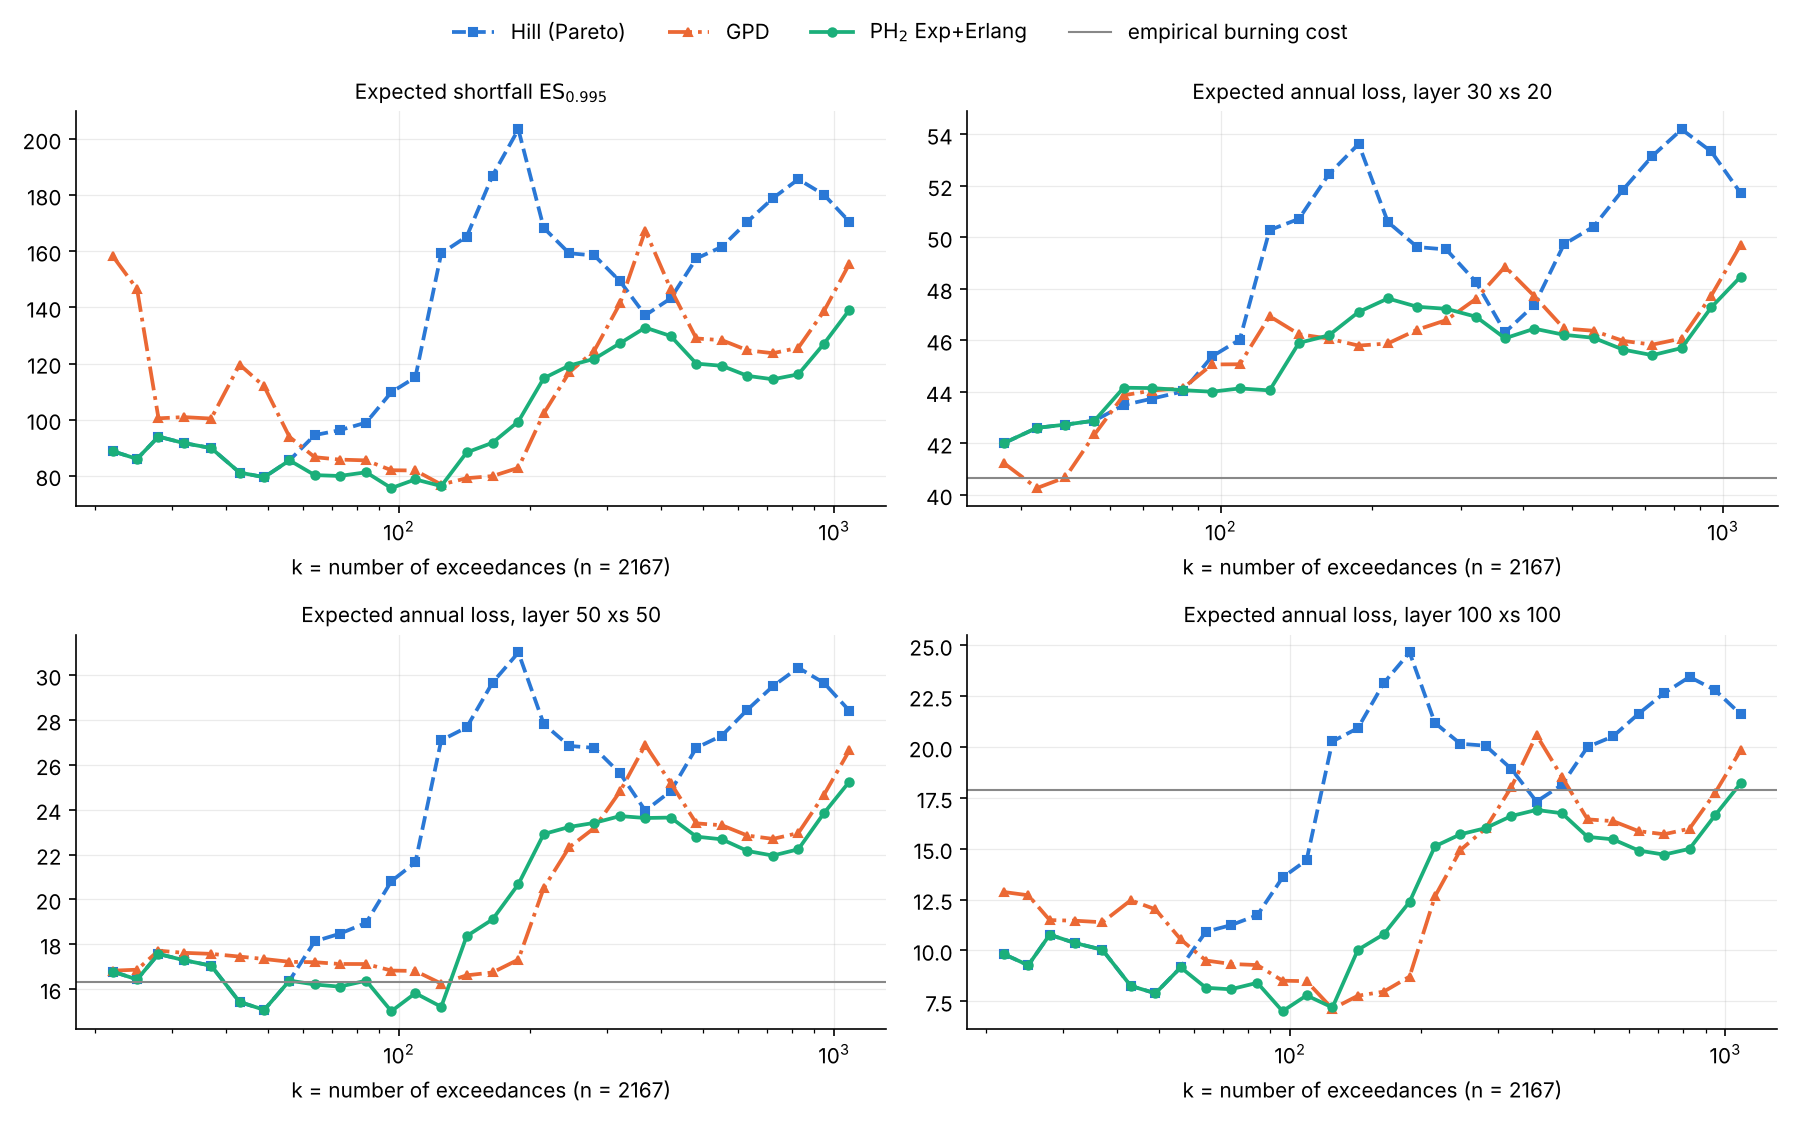
\includegraphics[width=\linewidth]{figures/danish_risk.png}
\caption{Danish fire losses: $\mathrm{ES}_{0.995}$ and expected annual loss in three excess-of-loss layers (millions of DKK) against the number of exceedances $k$, for the Pareto (Hill), GPD and E+E tails. Horizontal lines: empirical burning cost per year.}
\label{fig:danishrisk}
\end{figure}

\begin{table}[t]
\centering
\footnotesize
\setlength{\tabcolsep}{4pt}
\caption{Danish fire losses: expected shortfall and expected annual loss in three excess-of-loss layers (millions of DKK), with 95\% profile-likelihood intervals, at three thresholds.}
\label{tab:danishrisk}
\begin{tabular}{llrrr}
\toprule
Quantity & Method & $k=109$ ($u=9.9$) & $k=246$ ($u=5.1$) & $k=482$ ($u=3.2$) \\
\midrule
$\mathrm{ES}_{0.995}$ & Hill & 115.1 (70.3, 247.9) & 159.3 (96.6, 320.9) & 157.4 (104.7, 262.1) \\
 & GPD & 81.9 (54.0, 234.1) & 116.8 (63.3, 476.3) & 128.9 (72.3, 337.8) \\
 & E+E & 78.7 (53.7, 197.0) & 119.3 (72.3, 297.7) & 120.0 (73.2, 251.6) \\
\addlinespace
$\mathrm{ES}_{0.999}$ & Hill & 317.8 (163.9, 850.7) & 497.5 (264.5, 1170.4) & 489.1 (295.7, 906.6) \\
 & GPD & 182.5 (95.3, 823.4) & 321.6 (132.4, 1939.2) & 374.0 (170.5, 1265.0) \\
 & E+E & 172.8 (101.0, 637.3) & 327.1 (167.1, 1069.5) & 333.8 (173.6, 863.2) \\
\addlinespace
Layer 30 xs 20 [40.7] & Hill & 46.03 (32.38, 63.13) & 49.62 (35.72, 67.30) & 49.73 (37.06, 65.68) \\
 & GPD & 45.07 (31.75, 61.90) & 46.41 (31.68, 65.93) & 46.46 (31.76, 65.86) \\
 & E+E & 44.13 (30.72, 61.19) & 47.30 (33.05, 65.67) & 46.22 (31.95, 64.42) \\
\addlinespace
Layer 50 xs 50 [16.3] & Hill & 21.65 (11.73, 37.31) & 26.85 (16.62, 41.80) & 26.76 (17.92, 39.07) \\
 & GPD & 16.80 (7.43, 33.83) & 22.32 (10.44, 42.15) & 23.39 (12.33, 40.76) \\
 & E+E & 15.81 (7.27, 32.83) & 23.23 (12.67, 40.24) & 22.80 (12.61, 38.06) \\
\addlinespace
Layer 100 xs 100 [17.9] & Hill & 14.44 (6.28, 30.19) & 20.16 (10.99, 35.30) & 20.01 (12.24, 31.81) \\
 & GPD & 8.49 (1.90, 26.81) & 14.94 (4.62, 37.32) & 16.45 (6.76, 34.68) \\
 & E+E & 7.79 (2.42, 25.39) & 15.71 (6.78, 33.64) & 15.59 (7.01, 30.80) \\
\bottomrule
\end{tabular}
\par\smallskip
\parbox{\linewidth}{\footnotesize Layer entries are expected annual losses, i.e.\ the expected loss per claim in the layer times the observed claim frequency ($2167/11\approx197$ claims per year); the empirical burning cost per year is shown in square brackets. Intervals are conditional on the threshold and on the exceedance proportion $k/n$.}
\end{table}

\begin{table}[t]
\centering
\footnotesize
\setlength{\tabcolsep}{4pt}
\caption{Danish fire losses: standard deviation of each risk-measure estimate across the thresholds of Figure~\ref{fig:danishrisk}, by threshold window (smallest in bold).}
\label{tab:danishrisksd}
\begin{tabular}{lrrrrrrrrr}
\toprule
 & \multicolumn{3}{c}{all ($k=22$--$1084$)} & \multicolumn{3}{c}{$k=50$--$200$} & \multicolumn{3}{c}{$k=200$--$1084$} \\
\cmidrule(lr){2-4} \cmidrule(lr){5-7} \cmidrule(lr){8-10}
Quantity & Hill & GPD & E+E & Hill & GPD & E+E & Hill & GPD & E+E \\
\midrule
$\mathrm{ES}_{0.995}$ & 39.71 & 27.01 & \textbf{20.27} & 43.06 & \textbf{4.80} & 7.53 & 14.48 & 17.10 & \textbf{7.75} \\
$\mathrm{ES}_{0.999}$ & 157.58 & 118.54 & \textbf{78.41} & 173.58 & \textbf{23.96} & 26.81 & 56.70 & 71.43 & \textbf{32.48} \\
Layer 30 xs 20 & 3.96 & 2.34 & \textbf{1.75} & 4.08 & 1.37 & \textbf{1.29} & 2.36 & 1.22 & \textbf{0.90} \\
Layer 50 xs 50 & 5.42 & 3.59 & \textbf{3.48} & 5.36 & \textbf{0.33} & 1.84 & 1.90 & 1.78 & \textbf{0.89} \\
Layer 100 xs 100 & 5.60 & 3.91 & \textbf{3.67} & 5.68 & \textbf{0.98} & 1.71 & 1.83 & 2.11 & \textbf{1.01} \\
\bottomrule
\end{tabular}
\par\smallskip
\parbox{\linewidth}{\footnotesize Layers are evaluated only at thresholds below the retention.}
\end{table}


\section{Discussion and recommendations}\label{sec:discussion}

The two-phase phase-type class fitted to log-excesses has a transparent structure. Its two sub-families correspond exactly to the two second-order regimes, $\rho=0$ and $\rho<0$, of a regularly varying tail, and the rate parameters are invariant to the threshold. These properties explain why a PH$_2$ fit can be much more stable across thresholds than the Hill estimator or a GPD fit.

The simulation evidence, however, points to a more specific conclusion than the one suggested by the theory alone. The useful part of the PH$_2$ class is the Exp+Erlang sub-model, a two-parameter Pareto--log-gamma tail that generalises the Hill model by a single log factor. It competes with the GPD at the same number of parameters. It tolerates much lower thresholds than the Hill estimator, because its log factor absorbs slowly decaying second-order bias, and much smaller exceedance counts than the GPD, because it is fitted on the log scale where the data are better behaved. The two-exponential sub-family adds little: it is weakly identified, harms accuracy when selected, and does not recover $\rho$.

For practitioners we suggest the following.
\begin{enumerate}
\item Plot the E+E tail index estimate against the threshold, with profile-likelihood bands, alongside the Hill and GPD estimates. Choose the tail index from the region in which the E+E estimate is stable. As in \citet{KimKim2015}, this region typically begins at a much lower threshold than for the Hill plot.
\item If the E+E fit gives $\hat p$ close to zero over the stable region, the data are consistent with a nearly exact Pareto tail. The Hill estimator is then preferable because of its smaller variance (Proposition~\ref{prop:singular}).
\item Apply the min-shift of \citet{KimKim2015} only when the support of the losses demonstrably starts away from zero.
\item Do not interpret the PH$_2$ sub-family selected by AIC or BIC, or a fitted $\tau$, as an estimate of the second-order parameter. If $\rho$ is of interest, use a dedicated estimator \citep{FragaAlves2003,Goegebeur2010}.
\item For capital and reinsurance work, report expected shortfall and layer premiums from the E+E tail together with their profile-likelihood intervals (Section~\ref{sec:riskci}), and compare them across thresholds and with the GPD and Pareto values. The spread across thresholds and methods is a direct measure of the model risk that the threshold choice introduces.
\end{enumerate}

From an actuarial point of view, the E+E tail is a convenient replacement for the Pareto or GPD tail in a spliced severity model \citep{Reynkens2017}. It keeps closed-form layer premiums and expected shortfall, adds one parameter that absorbs slowly decaying second-order behaviour, and reduces to the Pareto tail when that parameter is not needed.

Several limitations should be noted. Our simulation covers one tail index ($\alpha=2$) and two sample sizes; tails heavier or lighter than this should be examined. The DGPs supported near zero (GPD, Burr) show that a log-scale method should not be pushed to thresholds in the body of the distribution. Finally, a formal test of $\rho=0$ against $\rho<0$ within the PH$_2$ family would require handling a boundary parameter, an unidentified nuisance parameter and a singular information matrix at once. A parametric bootstrap of the likelihood ratio is a natural candidate, which we leave for future work, together with extensions to inhomogeneous phase-type models \citep{AlbrecherBladt2019}.

\section*{Acknowledgements}
\todo{To be added.}

\section*{Disclosure statement}
No potential conflict of interest was reported by the author(s). \todo{Confirm.}

\section*{Funding}
\todo{Funding information, or delete this section if there was no funding.}

\section*{Data availability statement}\label{sec:availability}
The Danish fire insurance losses analysed in Section~\ref{sec:data} are publicly available, for example as the data set \texttt{danish} in the R package \texttt{evir}. All simulation code, raw per-sample estimates, summary tables, the risk-measure and interval code, and the scripts that produce every table and figure in this paper are available at \todo{repository URL or supplementary material}.

\bibliographystyle{apalike}
\bibliography{refs}

\appendix

\section{Proofs}\label{app:proofs}

\begin{proof}[Proof of Lemma~\ref{lem:eigen}]
Write $T=\begin{pmatrix}-\lambda_1&q_1\\q_2&-\lambda_2\end{pmatrix}$ with $\lambda_i>0$ and $0\le q_i\le\lambda_i$. The characteristic polynomial is $\psi^2+(\lambda_1+\lambda_2)\psi+\lambda_1\lambda_2-q_1q_2$, with discriminant $(\lambda_1-\lambda_2)^2+4q_1q_2\ge0$, so both roots are real. Their sum $-(\lambda_1+\lambda_2)$ is negative, and their product $\lambda_1\lambda_2-q_1q_2$ is positive because absorption is certain, which rules out $q_1=\lambda_1$ and $q_2=\lambda_2$ simultaneously. Hence both roots are negative.
\end{proof}

\begin{proof}[Proof of Proposition~\ref{prop:ph2}]
($\Rightarrow$) If $T$ has distinct eigenvalues $-\theta>-(\theta+\tau)$, then $e^{Tx}=e^{-\theta x}P_1+e^{-(\theta+\tau)x}P_2$ for the spectral projections $P_1,P_2$, so $S(x)=\beta e^{Tx}\mathbf 1=c_1e^{-\theta x}+c_2e^{-(\theta+\tau)x}$ with $c_1+c_2=S(0)=1$. Put $c_1=1-w$ and $c_2=w$. Since $f=-S'$ is a density, $f(0)=\theta+w\tau\ge0$, giving $w\ge-\theta/\tau$. As $x\to\infty$, $f(x)\sim(1-w)\theta e^{-\theta x}$ unless $w=1$, so $w\le1$. If $T$ has a double eigenvalue $-\mu$, then $T=-\mu I+N$ with $N^2=0$, so $e^{Tx}=e^{-\mu x}(I+Nx)$ and $S(x)=e^{-\mu x}(1+cx)$ with $c=\beta N\mathbf 1$. Writing $c=p\mu$ gives $f(x)=\mu e^{-\mu x}(1-p+p\mu x)$; nonnegativity at $x=0$ gives $p\le1$ and nonnegativity as $x\to\infty$ gives $p\ge0$.

($\Leftarrow$) For \eqref{eq:cox2E} the absorption time is $\mathrm{Exp}(\theta+\tau)$ with probability $1-q$ and the sum of independent $\mathrm{Exp}(\theta+\tau)$ and $\mathrm{Exp}(\theta)$ variables with probability $q$. Its density is
\[
(1-q)(\theta+\tau)e^{-(\theta+\tau)x}+q\,\frac{\theta(\theta+\tau)}{\tau}\big(e^{-\theta x}-e^{-(\theta+\tau)x}\big).
\]
The coefficient of $\theta e^{-\theta x}$ is $q(\theta+\tau)/\tau=1-w$, and that of $(\theta+\tau)e^{-(\theta+\tau)x}$ is $1-q-q\theta/\tau=w$, as required. Finally, $q\le1$ if and only if $w\ge-\theta/\tau$, and $q\ge0$ if and only if $w\le1$. The EE case is the same computation with $\theta+\tau$ and $\theta$ both replaced by $\mu$: the absorption time is $\mathrm{Exp}(\mu)$ with probability $1-p$ and $\mathrm{Erlang}(2,\mu)$ with probability $p$.
\end{proof}

\begin{proof}[Proof of Corollary~\ref{cor:tails}]
$\Pr(Y>y\mid Y>u_0)=S(\log(y/u_0))$ with $S$ from Proposition~\ref{prop:ph2}. The density of \eqref{eq:tailEE} is $(1-p)\mu u_0^{\mu}y^{-\mu-1}+p\mu^2u_0^{\mu}y^{-\mu-1}\log(y/u_0)$, the stated mixture.
\end{proof}

\begin{proof}[Proof of Theorem~\ref{thm:2rv}]
(a) With $s=\log(t/u_0)$, $\bF(tx)/\bF(t)=x^{-\mu}\{1+p\mu(s+\log x)\}/(1+p\mu s)=x^{-\mu}\{1+A(t)\log x\}$, which gives \eqref{eq:AEE}. Here $A(t)\to0$ and $A$ is slowly varying, so $\rho=0$.
(b) With $D(t)=1-w+we^{-\tau s}>0$,
\[
\frac{\bF(tx)}{\bF(t)}-x^{-\theta}=x^{-\theta}\Big\{\frac{1-w+we^{-\tau s}x^{-\tau}}{D(t)}-1\Big\}=x^{-\theta}\frac{we^{-\tau s}(x^{-\tau}-1)}{D(t)},
\]
which equals $A(t)x^{-\theta}(x^{-\tau}-1)/(-\tau)$ with $A$ as in \eqref{eq:A2E}. Since $D(t)\to1-w>0$, $A(t)\sim-\tau w(1-w)^{-1}(t/u_0)^{-\tau}$, so $|A|\in RV_{-\tau}$ and its sign is that of $-w$.
(c) is immediate.
\end{proof}

\begin{proof}[Proof of Corollary~\ref{cor:range}]
By Theorem~\ref{thm:2rv}, case (EE) with $p>0$ gives $\rho=0$, and case (2E) gives $\rho=-\tau$, where $\tau>0$ is arbitrary; the remaining cases are exactly Pareto.
\end{proof}

\begin{proof}[Proof of Proposition~\ref{prop:hill}]
The first statement is \eqref{eq:excess} applied to the representations of Proposition~\ref{prop:ph2}, with the weights obtained from $S(d+x)/S(d)$. (a) Under \eqref{eq:EE} with weight $p_d$, $\E E=(1-p_d)/\mu+2p_d/\mu=(1+p_d)/\mu$, and $p_d=p/(1+p\mu d)\sim1/(\mu\log u)$. (b) Under \eqref{eq:2E} with weight $w_d$, $\E E=(1-w_d)/\theta+w_d/(\theta+\tau)=\xi-\xi w_d\tau/(\theta+\tau)$, and $w_d=O(e^{-\tau d})=O(u^{-\tau})$. Consistency of the MLE at a fixed threshold follows because the log-excesses are i.i.d.\ from a member of the sub-model with the same rate parameters, and standard MLE theory applies in the interior of the parameter space; at the boundary $p_d=0$ (exact Pareto) consistency still holds since the Hill estimator is then the restricted MLE.
\end{proof}

\begin{proof}[Proof of Proposition~\ref{prop:fisher}]
Let $Z=\mu E$ and $D=1-p+pZ$. The density of $Z$ is $D\,e^{-z}$, $z>0$. Differentiating \eqref{eq:loglik} for one observation gives
\[
\partial_\mu^2\ell=-\mu^{-2}(1+p^2Z^2/D^2),\qquad \partial_\mu\partial_p\ell=\mu^{-1}Z/D^2,\qquad \partial_p^2\ell=-(Z-1)^2/D^2 .
\]
Since $D=p(a+Z)$, for any $g$ we have $\E[g(Z)/D^2]=p^{-1}\int_0^\infty g(z)e^{-z}(a+z)^{-1}dz$. Using $\int_0^\infty e^{-z}(a+z)^{-1}dz=J$, $\int_0^\infty ze^{-z}(a+z)^{-1}dz=1-aJ$ and $\int_0^\infty z^2e^{-z}(a+z)^{-1}dz=1-a+a^2J$, and noting $1+a=1/p$, we obtain \eqref{eq:fisher}. For $0<p<1$ the model is regular, and asymptotic normality of $(\hat\mu,\hat p)$ and the delta method for $\xi=1/\mu$ give the variance stated. Finally, $[I^{-1}]_{11}\mu^2$ depends on $p$ only, since $I_{11}\propto\mu^{-2}$, $I_{12}\propto\mu^{-1}$ and $I_{22}$ is free of $\mu$.
\end{proof}

\begin{proof}[Proof of Proposition~\ref{prop:risk}]
(a) With $r=y/u$, $\Pi_u(d)=\int_d^\infty\Pr(Y>y\mid Y>u)\,dy=u\int_a^\infty r^{-\mu}(1+p\mu\log r)\,dr$. For $\mu>1$, $\int_a^\infty r^{-\mu}dr=a^{1-\mu}/(\mu-1)$, and integration by parts gives
\[
\int_a^\infty r^{-\mu}\log r\,dr=\frac{a^{1-\mu}\log a}{\mu-1}+\frac{a^{1-\mu}}{(\mu-1)^2},
\]
which yields \eqref{eq:stoploss}. (b) $e(d)=\Pi_u(d)/\Pr(Y>d\mid Y>u)$, and dividing \eqref{eq:stoploss} by $a^{-\mu}(1+p\mu\log a)$ gives \eqref{eq:meanexcess}. (c) Since $\Pr(Y>y)=\pi_u\Pr(Y>y\mid Y>u)$ for $y\ge u$, the VaR equation follows. Then $\mathrm{ES}_q=v_q+\E[(Y-v_q)_+]/(1-q)$ for a continuous distribution, and $\E[(Y-v_q)_+]=\pi_u\Pi_u(v_q)$. (d) $\E[\min\{(Y-d)_+,L\}]=\E[(Y-d)_+]-\E[(Y-d-L)_+]$, and both terms equal $\pi_u\Pi_u(\cdot)$ for retentions at or above $u$.
\end{proof}

\begin{proof}[Proof of Proposition~\ref{prop:singular}]
Use the asymptotic series $J=e^aE_1(a)=\sum_{j\ge0}(-1)^jj!\,a^{-j-1}$ as $a\to\infty$, with $1/a=p/(1-p)=\sum_{i\ge1}p^i$. Collecting powers of $p$ gives $J=p+p^3-2p^4+9p^5+O(p^6)$. Hence
\[
\mu^2I_{11}=1+2p^2+O(p^3),\qquad \mu I_{12}=-(1-p+3p^2)+O(p^3),\qquad I_{22}=1-2p+9p^2+O(p^3),
\]
and $\mu^2\det I=(1+2p^2)(1-2p+9p^2)-(1-p+3p^2)^2+O(p^3)=4p^2+O(p^3)$. Then $\sigma^2_\xi/\xi^2=\mu^2[I^{-1}]_{11}=I_{22}/(\mu^2\det I)=\{4p^2\}^{-1}\{1+O(p)\}$. The scores at $p=0$ are $\partial_\mu\ell=\mu^{-1}-E$ and $\partial_p\ell=\mu E-1$, which are collinear. We confirmed the expansion numerically in 60-digit arithmetic.
\end{proof}

\section{Computational details}\label{app:computing}

For the 2E sub-family we use $\theta=e^{a}$, $\tau=e^{b}$ and $w=-\theta/\tau+(1+\theta/\tau)\,\mathrm{expit}(c)$, which maps $\mathbb R^3$ onto the full parameter range of Proposition~\ref{prop:ph2}. The log-likelihood is $-\theta\sum_jE_j+\sum_j\log\{(1-w)\theta+w(\theta+\tau)e^{-\tau E_j}\}$. For EE we use $\mu=e^{a}$ and $p=\mathrm{expit}(c)$. Both likelihoods are maximised by L-BFGS-B with analytic gradients from 18 (2E) and 9 (EE) starting values centred at the Hill estimate. The GPD is fitted by Nelder--Mead from three starting values. One replication with ten thresholds takes about one second at $n=2000$ on a single core.
\end{document}
